\chapter{Poligoni}
\label{chp:polygons}

Kako Weisstein tvrdi u~\cite{bib:Weisstein_polygon}, u literaturi nije usuglašena definicija poligona. Za potrebe ovog rada poligon će stoga biti definiran definicijom~\ref{def:polygon}, to jest, u nasatvku rada \emph{poligon} označava skup koji zadovoljava definiciju~\ref{def:polygon}.

\par

\begin{definition} \label{def:polygon}
    Za skup $ P \subseteq \reals^{\numprint{2}} $ kažemo da je \defined{poligon} ako vrijedi
    \begin{enumerate}
        \item \label{itm:polygon_bounded} $ P $ je ograničen,
        \item \label{itm:polygon_simple_closed_boundary} $ \boundary P $ je jednostavna zatvorena krivulja,
        \item \label{itm:polygon_finite} postoje $ k \in \naturals $ i točke $ V_{\numprint{1}} , V_{\numprint{2}} , \dotsc , V_{k} \in \reals^{\numprint{2}} $ takvi da je
        \begin{equation*}
            \boundary P = \linesegment{V_{\numprint{1}}}{V_{\numprint{2}}} \cup \linesegment{V_{\numprint{2}}}{V_{\numprint{3}}} \cup \dotsb \cup \linesegment{V_{k - \numprint{1}}}{V_{k}} \cup \linesegment{V_{k}}{V_{\numprint{1}}} \text{,}
        \end{equation*}
        pri čemu dužine u gornjoj uniji u parovima nemaju zajedničkih točaka osim eventualno krajnjih.
    \end{enumerate}
    Ako je $ P $ poligon i ako $ k \in \naturals $ zadovoljava točku~\ref{itm:polygon_finite}, onda za $ P $ kažemo da je \defined{$ k $-gon}. Ako je pritom $ k $ najmanji takav, onda za $ P $ kažemo da je \defined{pravi $ k $-gon}.

    \par

    Za poligon $ P $ točke $ V_{\numprint{1}} , V_{\numprint{2}} , \dotsc , V_{k} $ iz točke~\ref{itm:polygon_finite} zovemo \defined{vrhovima poligona $ P $}, a dužine $ \linesegment{V_{\numprint{1}}}{V_{\numprint{2}}} , \linesegment{V_{\numprint{2}}}{V_{\numprint{3}}} , \dotsc , \linesegment{V_{k - \numprint{1}}}{V_{k}} , \linesegment{V_{k}}{V_{\numprint{1}}} $ zovemo \defined{bridovima poligona $ P $}. Za $ i , j \in \left\{ \numprint{1} , \numprint{2} , \dotsc , k \right\} $ za vrhove $ V_{i} , V_{j} $ poligona $ P $ kažemo da su \defined{susjedni u poligonu $ P $} ako su različite krajnje točke istog brida poligona $ P $. Za dva brida poligona $ P $ kažemo da su \defined{susjedni u poligonu $ P $} ako imaju točno jednu zajedničku krajnju točku. Za $ i , j \in \left\{ \numprint{1} , \numprint{2} , \dotsc , k \right\} $ za dužine $ \linesegment{V_{i}}{V_{j}} $ koje nisu bridovi poligona $ P $ kažemo da su \defined{dijagonale poligona $ P $}.
\end{definition}

\par%
\clearpage%
\newpage

\begin{figure}[htb!]
    \centering
    \begin{subfigure}{0.3\textwidth}
        \centering
        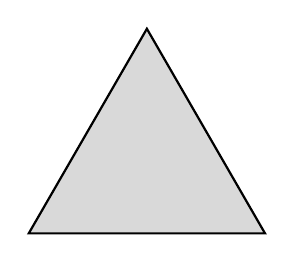
\begin{tikzpicture}[scale = 3]
            \filldraw[fill = black, fill opacity = 0.15, draw = black, thick] (0.5, -0.288675134594813) -- (0.0, 0.577350269189626) -- (-0.5, -0.288675134594813) -- cycle;
        \end{tikzpicture}
        \caption{\ding{51} Pravi \ensuremath{\numprint{3}}-gon}
        \label{fig:polygons_and_nonpolygons_polygon_1}
    \end{subfigure}
    \begin{subfigure}{0.3\textwidth}
        \centering
        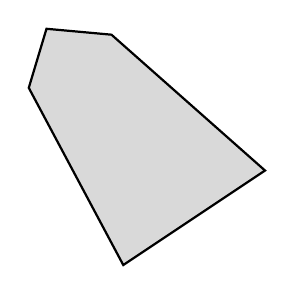
\begin{tikzpicture}[scale = 1.5]
            \filldraw[fill = black, fill opacity = 0.15, draw = black, thick] (-0.2, -1) -- (1, -0.2) -- (-0.3, 0.95) -- (-0.85, 1) -- (-1, 0.5) -- cycle;
        \end{tikzpicture}
        \caption{\ding{51} Pravi \ensuremath{\numprint{5}}-gon}
        \label{fig:polygons_and_nonpolygons_polygon_2}
    \end{subfigure}
    \begin{subfigure}{0.3\textwidth}
        \centering
        
\begin{tikzpicture}[scale = 1.5]
            \filldraw[fill = black, fill opacity = 0.15, draw = black, thick] (-1, -1) -- (0.25, -0.6) -- (0.40, -0.8) -- (0.55, -0.5) -- (1, -0.65) -- (0.45, 0) -- (-0.3, -0.2) -- (0.45, 1) -- (-0.6, -0.4) -- (-0.3, -0.35) -- cycle;
        \end{tikzpicture}
        \caption{\ding{51} Pravi \ensuremath{\numprint{10}}-gon}
        \label{fig:polygons_and_nonpolygons_polygon_3}
    \end{subfigure}
    \begin{subfigure}{0.3\textwidth}
        \centering
        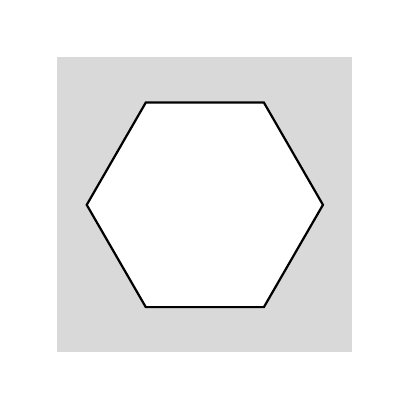
\begin{tikzpicture}[scale = 1.5]
            % Skup.
            \scope
                % Maska.
                \clip (-1.5, -1.5) rectangle (1.5, 1.5) (0.5, -0.866025403784439) -- (1, 0) -- (0.5, 0.866025403784439) -- (-0.5, 0.866025403784439) -- (-1, 0) -- (-0.5, -0.866025403784439) -- cycle;

                % Osjencani dio.
                \fill[black, opacity = 0.15] (-1.25, -1.25) rectangle (1.25, 1.25);
            \endscope

            % Rub skupa.
            \draw[black, thick] (0.5, -0.866025403784439) -- (1, 0) -- (0.5, 0.866025403784439) -- (-0.5, 0.866025403784439) -- (-1, 0) -- (-0.5, -0.866025403784439) -- cycle;
        \end{tikzpicture}
        \caption{\ding{55} Neograničeni skup}
        \label{fig:polygons_and_nonpolygons_nonpolygon_1}
    \end{subfigure}
    \begin{subfigure}{0.3\textwidth}
        \centering
        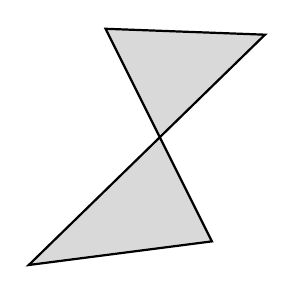
\begin{tikzpicture}[scale = 1.5]
            \filldraw[fill = black, fill opacity = 0.15, draw = black, thick] (-1, -1) -- (0.55, -0.8) -- (-0.35, 1) -- (1, 0.95) -- cycle;
        \end{tikzpicture}
        \caption{\ding{55} Rub nije jednostavna zatvorena krivulja}
        \label{fig:polygons_and_nonpolygons_nonpolygon_2}
    \end{subfigure}
    \begin{subfigure}{0.3\textwidth}
        \centering
        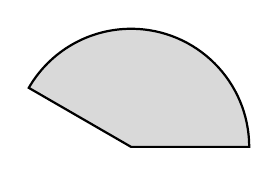
\begin{tikzpicture}[scale = 1.5]
            \filldraw[fill = black, fill opacity = 0.15, draw = black, thick] (1, 0) arc (0:150:1) -- (0, 0) -- cycle;
        \end{tikzpicture}
        \caption{\ding{55} Rub nije unija dužina}
        \label{fig:polygons_and_nonpolygons_nonpolygon_3}
    \end{subfigure}
    \caption[Primjeri poligona i skupova koji nisu poligoni]{Primjeri poligona i skupova koji nisu poligoni (u svrhu jednostavnosti skica izostavljeni su koordinatni sustavi)}
    \label{fig:polygons_and_nonpolygons}
\end{figure}

\par

Primjeri nekih skupova koji jesu poligoni i koji nisu poligoni prikazani su na slici~\ref{fig:polygons_and_nonpolygons}. Po nekim definicijama u literaturi skup na slici~\ref{fig:polygons_and_nonpolygons_nonpolygon_2} bio bi poligon, međutim, u ovom radu takve skupove ne smatramo poligonima jer interior takvog skupa nije povezan. Slično bi se mogao konstruirati zatvoreni skup čiji interior jest povezan, ali čiji rub nije jednostavna zatvorena krivulja---na primjer, bilo kojem poligonu na slici~\ref{fig:polygons_and_nonpolygons} na bilo koji vrh \emph{nadodamo}, kao dio ruba, dužinu duljine različite od $ \numprint{0} $ kojoj je jedan kraj taj vrh, a ostatak dužine disjunktan s početnim poligonom---no, i takve skupove ne ćemo smatrati poligonima jer želimo da je svaka točka na rubu poligona gomilište njegova interiora (da vrijedi $ \closure{\interior P} = \closure{P} $ i $ \boundary \interior P = \boundary P = \boundary \closure{P} $---\seetxt~propoziciju~\ref{prop:polygon_monotonicity}). Osim primjera na slici~\ref{fig:polygons_and_nonpolygons_nonpolygon_3} moguće je i da rub skupa jest prikaziv kao unija dužina, ali da je ta unija nužno beskonačna.

\par

Zahtjev da su dužine u uniji ulančane i da u parovima nemaju zajedničkih točaka osim eventualno krajnjih u točki~\ref{itm:polygon_finite} u definiciji~\ref{def:polygon} naveden je samo da bi se osiguralo da navedena unija prikazuje \emph{točno jedan obilazak} ruba i da definicije susjednih vrhova odnosno bridova imaju smisla. Inače, ako su za neki skup zadovoljene točke~\ref{itm:polygon_bounded} i \ref{itm:polygon_simple_closed_boundary}, dovoljno je, za provjeru je li taj skup poligon, dokazati da mu je rub prikaziv kao konačna unija dužina. Naime, ako dužine imaju zajedničkih točaka osim krajnjih, dužine prvo poredamo u fiksni poredak i onda, zbog činjenice da je rub jednostavna zatvorena krivulja, odlučujemo i postupamo sljedećim redom
\begin{enumerate}
    \item one dužine koje su duljine $ \numprint{0} $ odbacujemo,
    \item one dužine koje su disjunktne s već \emph{obiđenim} dijelom ruba osim eventualno u krajnjim točkama zadržavamo,
    \item one dužine koje cijele \emph{obilaze} već \emph{obiđeni} dio ruba odbacujemo,
    \item ostale dužine \emph{razlamamo} na nove dužine tako da izbacujemo već \emph{obiđene} dijelove ruba,
\end{enumerate}
pri čemu u posljednje dvije točke, kao i u drugoj, dopuštamo da su krajnje točke nove dužine već \emph{obiđene} osim ako je ona duljine $ \numprint{0} $ (tada je odbacujemo). Kako je početna unija konačna, od svake dužine tim postupkom dobijemo konačni broj novih dužina pa je rezultantna kolekcija dužina također konačna. Budući da su odbačeni samo dijelovi koji \emph{ne pridonose} uniji (izolirane točke, to jest, dužine duljine $ \numprint{0} $, sigurno ne pridonose jer je krivulja jednostavna i zatvorena, a početna unija konačna), rezultantna kolekcija dužina ima jednaku uniju kao početna. Sada još zbog činjenice da je rub jednostavna zatvorena krivulja slijedi da se ta unija može poredati i u ulančani poredak.

\par

Jednostavna zatvorena krivulja ne može biti prazni skup, izolirana točka ili dužina, stoga ne postoje $ \numprint{0} $-goni, $ \numprint{1} $-goni ni $ \numprint{2} $-goni. Inače iz prethodnog odlomka, Jordanovog teorema i svojstava otvorenih i zatvorenih skupova slijede teorem~\ref{thm:Jordan_curve_polygon} i propozicija~\ref{prop:polygon_monotonicity}.

\par

\begin{theorem} \label{thm:Jordan_curve_polygon}
    Neka je $ \Gamma \subseteq \reals^{\numprint{2}} $ proizvoljna jednostavna zatvorena krivulja. Ako postoji $ k \in \naturals $ i zatvorene dužine $ I_{\numprint{1}} , I_{\numprint{2}} , \dotsc , I_{k} \subseteq \reals^{\numprint{2}} $ takve da je $ \Gamma = I_{\numprint{1}} \cup I_{\numprint{2}} \cup \dotsb \cup I_{k} $, onda postoji jedinstveni otvoreni poligon $ P \subseteq \reals^{\numprint{2}} $ takav da je
    \begin{equation}
        \boundary P = \Gamma \text{,}
    \end{equation}
    štoviše, ako je taj poligon $ P $ pravi $ l $-gon za neki $ l \in \naturals $, onda vrijedi i
    \begin{equation}
        l \leq k \text{.}
    \end{equation}
\end{theorem}

\par

\begin{proposition} \label{prop:polygon_monotonicity}
    Neka su $ P , Q \subseteq \reals^{\numprint{2}} $ proizvoljni. Ako je $ P $ poligon i vrijedi $ \interior P \subseteq Q \subseteq \closure{P} $, onda je i $ Q $ poligon, štoviše, vrijedi
    \begin{gather}
        \interior P = \interior Q \subseteq \closure{Q} = \closure{P} \text{,} \\
        \boundary \interior P = \boundary Q = \boundary \closure{P} \text{.}
    \end{gather}
\end{proposition}

\par

\begin{definition} \label{def:equivalency}
    Za poligone $ P , Q \subseteq \reals^{\numprint{2}} $ kažemo da je \defined{poligon $ Q $ istovrstan poligonu $ P $}, što označavamo s \defined{$ Q \equiv P $}, ako je
    \begin{equation}
        \boundary Q = \boundary P \text{.}
    \end{equation}
\end{definition}

\par

\begin{remark} \label{rem:equivalency_simmetry}
    Relacija istovrsnosti iz definicije~\ref{def:equivalency} relacija je ekvivalencije. Stoga ćemo koristiti i neusmjerene izraze poput \emph{poligoni $ P $ i $ Q $ su istovrsni}, što znači da vrijedi $ P \equiv Q $ odnosno $ Q \equiv P $. Isto tako, ako su u nekoj familiji poligona svi poligoni u parovima istovrsni, onda ćemo reći da \emph{su svi poligoni (u toj familiji poligona) istovrsni}.
\end{remark}

\par

Neka je $ P \subseteq \reals^{\numprint{2}} $ proizvoljni poligon. Budući da on po definiciji ima konačno mnogo vrhova, jasno je da u konačno mnogo koraka broj njegovih vrhova možemo reducirati tako da u svakom koraku odbacimo neki vrh koji je jednak nekom drugom vrhu ili je kolinearan sa svoja susjedna dva vrha. Broj vrhova više ne ćemo moći reducirati kada su svi vrhovi u parovima različiti i nijedna tri susjedna vrha nisu kolinearni. Baš zato što nijedna tri susjedna vrha ne će biti kolinearni, nekim drugim izborom njegovih vrhova nemoguće je ne obuhvatiti sve te vrhove jer, ako bi se jedan od njih mogao izbjeći, onda bi on i neka njegova okolina točaka na rubu poligona s obje njegove strane morali ležati na istom bridu, koji mora biti \emph{ravan}, to jest, dužina kao podskup pravca (on bi tada bio kolinearan sa svoja susjedna dva vrha). Ovime su dokazani sljedeći teorem i propozicija~\ref{prop:polygon_nonplanar_vertices}.

\par

\begin{theorem} \label{thm:polygon_unique_vertices}
    Neka je skup $ P \subseteq \reals^{\numprint{2}} $ proizvoljan. Ako je $ P $ poligon, onda
    \begin{enumerate}
        \item \label{itm:polygon_unique_vertices_existance} postoje jedinstveni $ k \in \naturals $ i u parovima različite točke $ V_{\numprint{1}} , V_{\numprint{2}} , \dotsc , V_{k} \in \reals^{\numprint{2}} $ tako da je $ S $ pravi $ k $-gon i da su mu tada $ V_{\numprint{1}} , V_{\numprint{2}} , \dotsc , V_{k} $ vrhovi,
        \item \label{itm:polygon_unique_vertices_ordering} uređena $ k $-torka $ \left( V_{i_{\numprint{1}}} , V_{i_{\numprint{2}}} , \dotsc , V_{i_{k}} \right) \in \reals^{\numprint{2} \times k} $, $ i_{\numprint{1}} , i_{\numprint{2}} , \dotsc , i_{k} \in \left\{ \numprint{1} , \numprint{2} , \dotsc , k \right\} $, vrhova iz točke~\ref{itm:polygon_unique_vertices_existance} tako da se svaki vrh pojavljuje točno jednom i da su oni poredani u pozitivnom smjeru jedinstvena je do na izbor vrha $ V_{i_{\numprint{1}}} $.
    \end{enumerate}
\end{theorem}

\par

\begin{remark} \label{rem:polygon_vertices_positive_order}
    Poredak vrhova $ \left( V_{i_{\numprint{1}}} , V_{i_{\numprint{2}}} , \dotsc , V_{i_{k}} \right) $ poligona $ P $ u pozitivnom smjeru spomenut u teoremu~\ref{thm:polygon_unique_vertices} znači da postoji pozitivno orijentirana parametrizacija $ \varphi \colon \intervalcc{\numprint{0}}{\numprint{1}} \to \reals^{\numprint{2}} $ ruba poligona $ P $ takva da je $ \varphi \left( \numprint{0} \right) = \varphi \left( \numprint{1} \right) $ i da je $ \restrict{\varphi}{\intervalco{\numprint{0}}{\numprint{1}}} $ injektivna za koju onda vrijedi $ \varphi^{{- \numprint{1}}} \left( V_{i_{\numprint{1}}} \right) < \varphi^{{- \numprint{1}}} \left( V_{i_{\numprint{2}}} \right) < \dotsb < \varphi^{{- \numprint{1}}} \left( V_{i_{k}} \right) $, gdje je $ \varphi^{{- \numprint{1}}} $ inverz restrikcije $ \restrict{\varphi}{\intervalco{\numprint{0}}{\numprint{1}}} $. Kada će se u ostatku rada spominjati da su vrhovi nekog poligona poredani ili enumerirani u pozitivnom smjeru, onda će to značiti
    \begin{itemize}
        \item ako su svi vrhovi u uređenoj kolekciji vrhova u parovima različiti, značenje je analogno značenju u teoremu~\ref{thm:polygon_unique_vertices} objašnjenom u prvom dijelu ove napomene (ali tako da po potrebi dopuštamo da su neka tri uzastopna vrha kolinearna),
        \item ako u uređenoj kolekciji vrhova postoje jednaki vrhovi, onda za svaki izbor u parovima različitih vrhova tako da se svaki vrh iz početne kolekcije pojavljuje barem jednom (dakle, točno jednom) njihov poredak naslijeđen iz originalne kolekcije mora biti u pozitivnom smjeru sa značenjem kao u prethodnoj točki.
    \end{itemize}
    Negativni poredak i negativna enumeracija značit će, jasno, da je obrnuti poredak odnosno \emph{obrnuta enumeracija} pozitivan/-na.
\end{remark}

\par

Uočimo da obratno teoremu~\ref{thm:polygon_unique_vertices} zadavanjem uređene $ k $-torke točaka u ravnini možemo zadati zatvorenu krivulju prikazivu kao ulančanu uniju dužina. Međutim, ona ne mora nužno biti jednostavna krivulja, taj izbor vrhova ne mora nužno biti ireducibilan (vrhovi se mogu ponavljati i neki vrh može biti kolinearan s oba njemu susjedna vrha) i, ako je krivulja jednostavna, zadani \emph{obilazak} krivulje ne mora biti u pozitivnom smjeru. Slijedi da je za svaki $ k \in \naturals $ preslikavanje iz klasa istovrsnih pravih $ k $-gona u skup $ \reals^{\numprint{2} \times k} $ s usuglašenim izborom prvog vrha (na primjer, prvi vrh je koordinatno leksikografski najmanji) injektivno, ali nije surjektivno.

\par

\begin{definition} \label{def:polygon_true_vertex}
    Neka je $ P \subseteq \reals^{\numprint{2}} $ poligon. Neka je $ k \in \naturals $ takav da je $ P $ pravi $ k $-gon. Za točku $ V \in \reals^{\numprint{2}} $/zatvorenu dužinu $ E \subseteq \reals^{\numprint{2}} $/zatvorenu dužinu $ D \subseteq \reals^{\numprint{2}} $ kažemo da je \defined{pravi vrh}/\defined{pravi brid}/\defined{prava dijagonala poligona $ P $} ako se pojavljuje kao vrh/brid/dijagonala poligona $ P $ promatranog kao pravi $ k $-gon.
\end{definition}

\par

\begin{proposition} \label{prop:polygon_nonplanar_vertices}
    Neka je skup $ P \subseteq \reals^{\numprint{2}} $ proizvoljan. Ako je $ P $ poligon, onda nijedna njegova tri uzastopna prava vrha u pozitivnom smjeru nisu kolinearni.
\end{proposition}

\par

Uzmimo sada proizvoljni $ k \in \naturals $ takav da je $ k \geq \numprint{3} $. U proizvoljnom $ k $-gonu bilo koji brid možemo podijeliti na proizvoljno konačno mnogo (ali barem $ \numprint{1} $) uzastopnih bridova koji leže na istom pravcu \emph{umetanjem} proizvoljno konačno mnogo vrhova, stoga svaki $ k $-gon možemo promatrati kao $ l $-gon za proizvoljni $ l \in \naturals $, $ l \geq k $. S druge strane, ako za svaki $ i \in \left\{ \numprint{1} , \numprint{2} , \dotsc , k \right\} $ definiramo točku $ V_{i} \coloneqq \left( \cos \left( \frac{\numprint{2} \left( i - \numprint{1} \right)}{k} \pi \right) , \sin \left( \frac{\numprint{2} \left( i - \numprint{1} \right)}{k} \pi \right) \right) \in \reals^{\numprint{2}} $, uočavamo da je $ \Gamma \coloneqq \linesegment{V_{\numprint{1}}}{V_{\numprint{2}}} \cup \linesegment{V_{\numprint{2}}}{V_{\numprint{3}}} \cup \dotsb \cup \linesegment{V_{k - \numprint{1}}}{V_{k}} \cup \linesegment{V_{k}}{V_{\numprint{1}}} \subseteq \reals^{\numprint{2}} $ jednostavna zatvorena krivulja, iz čega po teoremu~\ref{thm:Jordan_curve_polygon} pronalazimo $ l $-gon s rubom $ \Gamma $ za neki $ l \in \naturals $, $ l \leq k $. Lako se provjeri da nijedne tri definirane uzastopne točke (pri čemu uzimamo ciklički poredak, to jest, točka $ V_{k} $ prethodi točki $ V_{\numprint{1}} $) nisu na istom pravcu i da su točke enumerirane u pozitivnom smjeru, što ga čini i pravim $ k $-gonom. Konačno, zbog proizvoljnosti broja $ k $ zaključujemo da osim isključenih $ \numprint{0} $-gona, $ \numprint{1} $-gona i $ \numprint{2} $-gona svi ostali $ k $-goni postoje, pri čemu klase $ k $-gona rastu (s obzirom na relaciju inkluzije na klasama) za broj vrhova iz $ \naturals $, a strogo rastu za broj vrhova iz $ \naturals \setminus \left\{  \numprint{0} , \numprint{1} \right\} $ odnosno $ \naturals \setminus \left\{ \numprint{0} , \numprint{1} , \numprint{2} \right\} $. Kako je klasa $ \numprint{2} $-gona prazna, a klasa $ \numprint{3} $-gona nije prazna, slijedi i da je svaki $ \numprint{3} $-gon ujedno i pravi $ \numprint{3} $-gon.

\par

\begin{proposition} \label{prop:diameter_polygon}
    Neka je $ P \subseteq \reals^{\numprint{2}} $ proizvoljan. Ako je $ P $ poligon, onda postoje vrhovi $ V , W \in \reals^{\numprint{2}} $ poligona $ P $ takvi da vrijedi
    \begin{equation}
        \distance{V}{W} = \diameter \left( P \right) \text{.}
    \end{equation}
\end{proposition}

\par

\begin{proof}
    Neka je $ P \subseteq \reals^{\numprint{2}} $ proizvoljan. Pretpostavimo da je $ P $ poligon.

    \par

    Ideja dokaza je najprije prikazati da za proizvoljne točke na rubu poligona postoje dva vrha koji su međusobno udaljeniji od početne dvije točke. Nakon toga dokaz propozicije jednostavno će slijediti iz već dokazanih rezultata.

    \par

    \begin{figure}[htb!]
        \centering
        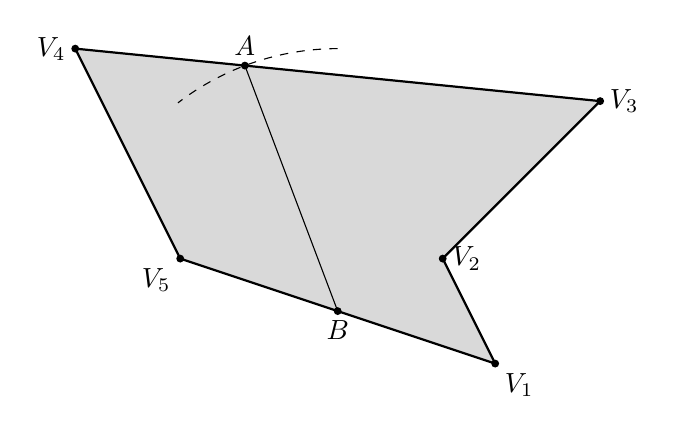
\begin{tikzpicture}[scale = 0.666666666666667]
            % Poligon.
            \filldraw[fill = black, fill opacity = 0.15, draw = black, thick] (3, -3) -- (2, -1) -- (5, 2) -- (-5, 3) -- (-3, -1) -- cycle;

            % Pomoćne linije.
            \draw[black, thin] (-1.76838413613841, 2.67683841361384) -- (0, -2);
            \draw[black, dashed] (0, 3) arc (90:127.5:5);

            % Vrhovi.
            \fill[black] (3, -3) circle (0.075) node[below right] {$ V_{\numprint{1}} $};
            \fill[black] (2, -1) circle (0.075) node[right] {$ V_{\numprint{2}} $};
            \fill[black] (5, 2) circle (0.075) node[right] {$ V_{\numprint{3}} $};
            \fill[black] (-5, 3) circle (0.075) node[left] {$ V_{\numprint{4}} $};
            \fill[black] (-3, -1) circle (0.075) node[below left] {$ V_{\numprint{5}} $};

            % Tocke A, B.
            \fill[black] (-1.76838413613841, 2.67683841361384) circle (0.075) node[above] {$ A $};
            \fill[black] (0, -2) circle (0.075) node[below] {$ B $};
        \end{tikzpicture}
        \caption[Pronalazak vrhova poligona koji su udaljeniji od točaka na rubu poligona]{Pronalazak vrhova poligona koji su udaljeniji od točaka na rubu poligona (u svrhu jednostavnosti skice izostavljen je koordinatni sustav). Vrh \ensuremath{V_{\numprint{4}}} očito je dobar kandidat za točku \ensuremath{A^{{*}}}, ali, kada bi se kružni luk proširio, bilo bi vidljivo da je i \ensuremath{\distance{V_{\numprint{3}}}{B} > \distance{A}{B}}.}
        \label{fig:diameter_polygon_distant_points}
    \end{figure}

    \par

    Neka su $ A , B \in \boundary P $ proizvoljne različite točke. Postupak koji slijedi ilustriran je na slici~\ref{fig:diameter_polygon_distant_points}. Ako je $ A $ vrh poligona $ P $, označimo $ A^{{*}} \coloneqq A $. U protivnom promatramo kružnicu radijusa $ \distance{A}{B} $ sa središtem u točki $ B $. Dvije su mogućnosti: brid kojem točka $ A $ pripada dodiruje promatranu kružnicu ili je siječe. U svakom slučaju postoji barem jedan vrh---jedna krajnja točka brida kojem pripada točka $ A $---koji se nalazi izvan otvorenog kruga kojeg promatrana kružnica \emph{zatvara}. Označimo tada jedan takav (ili jedinstveni ako je samo jedan) vrh s $ A^{{*}} $. Po konstrukciji je, neovisno o tomu je li $ A^{{*}} = A $ ili ne, $ \distance{A^{{*}}}{B} \geq \distance{A}{B} $. Sada analogno činimo s pronalaskom vrha $ B^{{*}} $, ali ovaj put središte kružnice postavljamo na $ A^{{*}} $, a ne na $ A $ (ako je $ A^{{*}} \neq A $). Konačno je $ \distance{A^{{*}}}{B^{{*}}} \geq \distance{A^{{*}}}{B} \geq \distance{A}{B} $. Zbog proizvoljnosti točaka $ A , B $ slijedi da za izbor svake dvije točke na $ \boundary P $ postoje dva vrha poligona $ P $ koji su međusobno udaljeniji (ne nužno strogo) od početne dvije točke (iako smo zadali ograničenje $ A \neq B $, ali za točke $ A = B $ njihova je udaljenost ionako najmanja moguća).

    \par

    Kako je vrhova poligona konačno mnogo, postoji maksimum udaljenosti njegovih vrhova i on se tada postiže na nekom paru vrhova poligona. Zbog definicione ograničenosti poligona (\seetxt~definiciju~\ref{def:polygon}), po propoziciji~\ref{prop:finite_diameter} i prethodno dokazanom sada slijedi tvrdnja propozicije.
\end{proof}

\par

Bitan je rezultat prethodne propozicije da je za računanje dijametra poligona dovoljno tražiti maksimum duljina njegovih stranica i dijagonala. To jest, ako su nam poznati položaji svih vrhova, dovoljno je izračunati $ \binom{k}{\numprint{2}} \in \bigO \left( k^{\numprint{2}} \right) $ njihovih međusobnih udaljenosti da bi se pronašla maksimalna, koja je tada dijametar poligona. Kako su funkcije kvadrata i korijena obje rastuće, za efikasno numeričko računanje maksimalne udaljenosti dovoljno je maksimizirati kvadratne udaljenosti. Kod euklidske udaljosti točaka čije su koordinate poznate maksimizacija kvadratnih udaljenosti jednostavna je, a na računalima je funkcija numeričkog korijenovanja obično \emph{skupa} i zato ju je efikasno primijeniti samo jednom---i to na maksimalnom kvadratu udaljenosti vrhova---za računanje dijametra poligona.

\par

Važno je za primijetiti da u propoziciji~\ref{prop:diameter_polygon} nije fiksiran nijedan izbor vrhova poligona. To zapravo znači da rezultat propozicije posebno vrijedi i ako poligon proučavamo kao pravi $ k $-gon kada je skup vrhova jedinstven i najmanji po inkluziji. Drugim riječima, dijametar poligona postiže se kao udaljenost nekih njegovih pravih vrhova.

\par

\begin{remark} \label{rem:polygon_name}
    U daljnjem dijelu rada, kada je broj vrhova poznat i bitan, koristit će se i uvaženi hrvatski nazivi, to jest, $ \numprint{3} $-goni će se zvati \emph{trokutima}, $ \numprint{4} $-goni \emph{četverokutima}{\ldots} Naziv $ k $-gon koristit će se uglavnom u kontekstu kada broj vrhova nije poznat odnosno nije bitan.
\end{remark}

\par

Rub poligona je, po definiciji, jednostavna zatvorena krivulja koja se može prikazati kao konačna (ulančana) unija dužina, a moguće ga je čak prikazati i kao uniju dužina duljine različite od $ \numprint{0} $. Svaka dužina može se prikazati kao slika afine funkcije na nekom segmentu, stoga, budući da su afine funkcije glatke, rub je svakog poligona po dijelovima gladak. Slijedi da svaki otvoreni poligon zadovoljava uvjete na skup iz definicije~\ref{def:Laplacian_eigen}, dakle, postoji spektar svakog otvorenog poligona.

\par

\section{Karakterizacija poligona}
\label{sec:polygon_characterisation}

Jednu karakterizaciju poligona već smo spomenuli, a to je, uz određene stupnjeve slobode, jedinstvena $ k $-torka vrhova poligona promatranog kao pravog $ k $-gona iz teorema~\ref{thm:polygon_unique_vertices}. Ta karakterizacija, doduše, nije pogodna za karakterizaciju domene u problemu računanja spektra iz sljedećih razloga:
\begin{itemize}
    \item ona ovisi o položaju poligona u ravnini,
    \item ona ovisi o rotaciji poligona u ravnini,
    \item ona ovisi o orijentaciji poligona u ravnini---ovo se može korigirati dopuštanjem da poredak vrhova bude i u negativnom smjeru,
    \item ona ovisi o dijametru poligona.
\end{itemize}
Osim navedenih manjkavosti, ova karakterizacija problematična je i zato što ona ovisi o izboru prvog vrha (ako dopuštamo da obilazak vrhova bude i u negativnom smjeru, onda ona ovisi i o izboru drugog vrha). Naime, zbog invarijantnosti na refleksije i neprekidnosti spektra (\seetxt~teoreme~\ref{thm:Laplacian_eigenvalue_similar_domains} i \ref{thm:Laplace_eigenvalue_continuity}) poželjno je da karakterizacija bude robusna na transformacije refleksijama i da bude neprekidna, stoga neke \emph{klasične konvencije} o izboru nisu dobre, što je vidljivo na slici~\ref{fig:polygon_minimal_change}. Konvencija enumeriranja vrhova na slici~\ref{fig:polygon_minimal_change} jest:
\begin{enumerate}
    \item prvi vrh (vrh $ V_{\numprint{1}} $/$ V_{\numprint{1}} ' $/$ V_{\numprint{1}} '' $) je vrh čije su koordinate leksikografski najmanje,
    \item enumeracija vrhova je u pozitivnom smjeru.
\end{enumerate}
Čak i da se prvi vrh (vrh $ V_{\numprint{1}} $/$ V_{\numprint{1}} ' $/$ V_{\numprint{1}} '' $) birao, na primjer, kriterijem najmanje druge koordinate (i najveće prve koordinate ako više vrhova ima istu i najmanju vrijednost druge koordinate), na slici~\ref{fig:polygon_minimal_change_vertex_displacement} vrh $ V_{\numprint{1}} '' $ ne bi bio onaj vrh koji \emph{odgovara} vrhu $ V_{\numprint{1}} $ na slici~\ref{fig:polygon_minimal_change_original}---vrh $ V_{\numprint{4}} '' $ na slici~\ref{fig:polygon_minimal_change_vertex_displacement}---nego onaj vrh koji \emph{odgovara} vrhu $ V_{\numprint{2}} $ na slici~\ref{fig:polygon_minimal_change_original}---vrh $ V_{\numprint{5}} '' $ na slici~\ref{fig:polygon_minimal_change_vertex_displacement}. Ipak, uz određene prethodne transformacije ta je karakterizacija u određenim slučajevima zadovoljavajuće dobra (zbog propozicije~\ref{prop:triangle_characteristic_bijective} koristit ćemo je, među ostalima, u daljnjem dijelu rada).

\par

\begin{figure}[htb!]
    \centering
    \begin{subfigure}{0.3\textwidth}
        \centering
        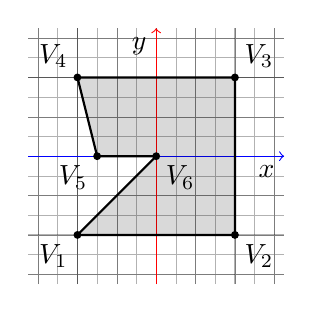
\begin{tikzpicture}
            % Koordinatna mreza.
            \draw[black, opacity = 0.3, very thin, step = 0.25] (-1.625, -1.625) grid (1.625, 1.625);
            \draw[black, opacity = 0.3, very thin, step = 0.5] (-1.625, -1.625) grid (1.625, 1.625);
            \draw[black, opacity = 0.3, thin, step = 1] (-1.625, -1.625) grid (1.625, 1.625);

            % Koordinatne osi.
            \draw[blue, thin, ->] (-1.625, 0) -- (1.625, 0) node[black, below left] {$ x $};
            \draw[red, thin, ->] (0, -1.625) -- (0, 1.625) node[black, below left] {$ y $};

            % Poligon.
            \filldraw[fill = black, fill opacity = 0.15, draw = black, thick] (1, -1) -- (1, 1) -- (-1, 1) -- (-0.75, 0) -- (0, 0) -- (-1, -1) -- cycle;

            % Vrhovi poligona.
            \fill[black] (-1, -1) circle (0.05) node[below left] {$ V_{\numprint{1}} $};
            \fill[black] (1, -1) circle (0.05) node[below right] {$ V_{\numprint{2}} $};
            \fill[black] (1, 1) circle (0.05) node[above right] {$ V_{\numprint{3}} $};
            \fill[black] (-1, 1) circle (0.05) node[above left] {$ V_{\numprint{4}} $};
            \fill[black] (-0.75, 0) circle (0.05) node[below left] {$ V_{\numprint{5}} $};
            \fill[black] (0, 0) circle (0.05) node[below right] {$ V_{\numprint{6}} $};
        \end{tikzpicture}
        \caption{Originalni poligon}
        \label{fig:polygon_minimal_change_original}
    \end{subfigure}
    \begin{subfigure}{0.3\textwidth}
        \centering
        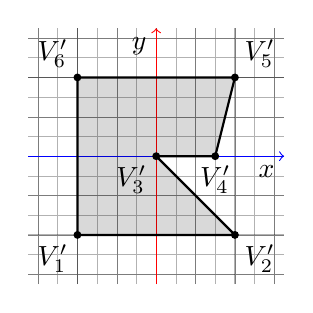
\begin{tikzpicture}
            % Koordinatna mreza.
            \draw[black, opacity = 0.3, very thin, step = 0.25] (-1.625, -1.625) grid (1.625, 1.625);
            \draw[black, opacity = 0.3, very thin, step = 0.5] (-1.625, -1.625) grid (1.625, 1.625);
            \draw[black, opacity = 0.3, thin, step = 1] (-1.625, -1.625) grid (1.625, 1.625);

            % Koordinatne osi.
            \draw[blue, thin, ->] (-1.625, 0) -- (1.625, 0) node[black, below left] {$ x $};
            \draw[red, thin, ->] (0, -1.625) -- (0, 1.625) node[black, below left] {$ y $};

            % Poligon.
            \filldraw[fill = black, fill opacity = 0.15, draw = black, thick] (1, -1) -- (0, 0) -- (0.75, 0) -- (1, 1) -- (-1, 1) -- (-1, -1) -- cycle;

            % Vrhovi poligona.
            \fill[black] (-1, -1) circle (0.05) node[below left] {$ V_{\numprint{1}} ' $};
            \fill[black] (1, -1) circle (0.05) node[below right] {$ V_{\numprint{2}} ' $};
            \fill[black] (0, 0) circle (0.05) node[below left] {$ V_{\numprint{3}} ' $};
            \fill[black] (0.75, 0) circle (0.05) node[below] {$ V_{\numprint{4}} ' $};
            \fill[black] (1, 1) circle (0.05) node[above right] {$ V_{\numprint{5}} ' $};
            \fill[black] (-1, 1) circle (0.05) node[above left] {$ V_{\numprint{6}} ' $};
        \end{tikzpicture}
        \caption{Refleksija oko ordinate}
        \label{fig:polygon_minimal_change_reflection}
    \end{subfigure}
    \begin{subfigure}{0.3\textwidth}
        \centering
        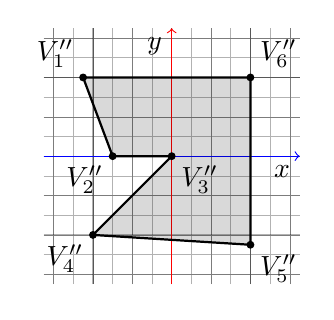
\begin{tikzpicture}
            % Koordinatna mreza.
            \draw[black, opacity = 0.3, very thin, step = 0.25] (-1.625, -1.625) grid (1.625, 1.625);
            \draw[black, opacity = 0.3, very thin, step = 0.5] (-1.625, -1.625) grid (1.625, 1.625);
            \draw[black, opacity = 0.3, thin, step = 1] (-1.625, -1.625) grid (1.625, 1.625);

            % Koordinatne osi.
            \draw[blue, thin, ->] (-1.625, 0) -- (1.625, 0) node[black, below left] {$ x $};
            \draw[red, thin, ->] (0, -1.625) -- (0, 1.625) node[black, below left] {$ y $};

            % Poligon.
            \filldraw[fill = black, fill opacity = 0.15, draw = black, thick] (1, -1.125) -- (1, 1) -- (-1.125, 1) -- (-0.75, 0) -- (0, 0) -- (-1, -1) -- cycle;

            % Vrhovi poligona.
            \fill[black] (-1.125, 1) circle (0.05) node[above left] {$ V_{\numprint{1}} '' $};
            \fill[black] (-0.75, 0) circle (0.05) node[below left] {$ V_{\numprint{2}} '' $};
            \fill[black] (0, 0) circle (0.05) node[below right] {$ V_{\numprint{3}} '' $};
            \fill[black] (-1, -1) circle (0.05) node[below left] {$ V_{\numprint{4}} '' $};
            \fill[black] (1, -1.125) circle (0.05) node[below right] {$ V_{\numprint{5}} '' $};
            \fill[black] (1, 1) circle (0.05) node[above right] {$ V_{\numprint{6}} '' $};
        \end{tikzpicture}
        \caption{\emph{Mali} pomak vrhova}
        \label{fig:polygon_minimal_change_vertex_displacement}
    \end{subfigure}
    \caption[Posljedice \emph{malih} promjena poligona na karakterizaciju poligona uređenom \ensuremath{k}-torkom vrhova]{Posljedice \emph{malih} promjena poligona na karakterizaciju poligona uređenom \ensuremath{k}-torkom vrhova. Najmanji razmak između linija \emph{mreže} koordinatnog sustava iznosi \ensuremath{\numprint{0.25}}, stoga vrh \ensuremath{V_{\numprint{1}}} na slici~\ref{fig:polygon_minimal_change_original}, na primjer, ima koordinate \ensuremath{\left( {- \numprint{1}} , \numprint{1} \right)}.}
    \label{fig:polygon_minimal_change}
\end{figure}

\par

\begin{definition} \label{def:outer_angle}
    Neka je $ k \in \naturals $, $ k \geq \numprint{3} $. Neka je $ P \subseteq \reals^{\numprint{2}} $ $ k $-gon. Neka su točke $ V_{\numprint{1}} , V_{\numprint{2}} , \dotsc , V_{k} \in \reals^{\numprint{2}} $ svi u parovima različiti vrhovi (u smislu da se među njima nalaze svi pravi vrhovi) poligona $ P $ enumerirani u pozitivnom smjeru. Označimo $ V_{\numprint{0}} \coloneqq V_{k} $ i $ V_{k + \numprint{1}} \coloneqq V_{\numprint{1}} $. Za $ i \in \left\{ \numprint{1} , \numprint{2} , \dotsc , k \right\} $ definiramo \defined{vanjski kut poligona $ P $ u vrhu $ V_{i} $} kao kut $ \varphi $ između vektora $ \vectorline{V_{i - \numprint{1}}}{V_{i}} $ i $ \vectorline{V_{i}}{V_{i + \numprint{1}}} $ tako da je $ \vectorline{V_{i - \numprint{1}}}{V_{i}} \cdot \vectorline{V_{i}}{V_{i + \numprint{1}}} = \left\lvert \vectorline{V_{i - \numprint{1}}}{V_{i}} \right\rvert \left\lvert \vectorline{V_{i}}{V_{i + \numprint{1}}} \right\rvert \cos \varphi $ čija je vrijednost u skupu $ \intervaloc{{- \pi}}{\pi} $, a predznak jednak predznaku determinante
    \begin{equation*}
        \begin{vmatrix}
            \numprint{1} & x_{i - \numprint{1}} & y_{i - \numprint{1}} \\
            \numprint{1} & x_{i} & y_{i} \\
            \numprint{1} & x_{i + \numprint{1}} & y_{i + \numprint{1}}
        \end{vmatrix}
        = \left( x_{i} - x_{i - \numprint{1}} \right) \left( y_{i + \numprint{1}} - y_{i - \numprint{1}} \right) - \left( x_{i + \numprint{1}} - x_{i - \numprint{1}} \right) \left( y_{i} - y_{i - \numprint{1}} \right) \in \reals \text{,}
    \end{equation*}
    gdje su $ \left( x_{i - \numprint{1}} , y_{i - \numprint{1}} \right) , \left( x_{i} , y_{i} \right) , \left( x_{i + \numprint{1}} , y_{i + \numprint{1}} \right) \in \reals^{\numprint{2}} $ redom koordinate vrhova $ V_{i - \numprint{1}} , V_{i} , V_{i + \numprint{1}} $ u kanonskoj bazi.
\end{definition}

\par

\begin{figure}[hbt!]
    \centering
    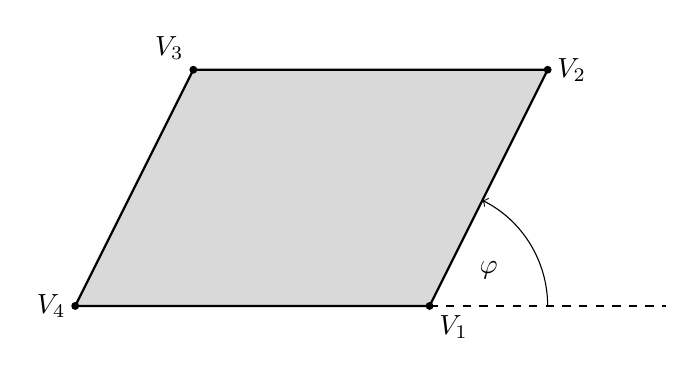
\begin{tikzpicture}[scale = 1.5]
        % Poligon.
        \filldraw[fill = black, fill opacity = 0.15, draw = black, thick] (1, -1) -- (2, 1) -- (-1, 1) -- (-2, -1) -- cycle;

        % Pomocni polupravac.
        \draw[black, dashed] (1, -1) -- (3, -1);

        % Vrhovi poligona.
        \fill[black] (1, -1) circle (0.033333333333333) node[below right] {$ V_{\numprint{1}} $};
        \fill[black] (2, 1) circle (0.033333333333333) node[right] {$ V_{\numprint{2}} $};
        \fill[black] (-1, 1) circle (0.033333333333333) node[above left] {$ V_{\numprint{3}} $};
        \fill[black] (-2, -1) circle (0.033333333333333) node[left] {$ V_{\numprint{4}} $};

        % Kruzni luk.
        \draw[black, ->] (2, -1) arc (0:63.434948822922011:1);

        % Kut.
        \draw[black] (1.5, -0.7) node {$ \varphi $};
    \end{tikzpicture}
    \caption[Vanjski kut u vrhu poligona]{Vanjski kut u vrhu poligona (u svrhu jednostavnosti skice izostavljen je koordinatni sustav). Ilustrirano je čemu je, zapravo, jednak vanjski kut definiran definicijom~\ref{def:outer_angle}, u vrhu \ensuremath{V_{\numprint{1}}} prikazanog paralelograma. Strelica pokazuje smjer u kojem se kut računa.}
    \label{fig:outer_angle}
\end{figure}

\par

Osim što po definiciji vrijednost vanjskog kuta ne može biti $ {- \pi} $, zbog činjenice da nijedna tri uzastopna prava vrha nisu kolinearni, vanjski kut u svakom pravom vrhu poligona nije ni $ \numprint{0} $ ni $ \pi $; naime, valja uočiti da bi vrijednost determinante u definiciji~\ref{def:outer_angle} bila jednaka $ \numprint{0} $ onda i samo onda kada bi sva tri vrha $ V_{i - \numprint{1}} , V_{i} , V_{i + \numprint{1}} $ bili kolinearni. Kad bi vanjski kut u nekom vrhu iznosio $ \pi $, onda bi on i njemu dva susjedna vrha bili kolinearni, ali bi oba njemu susjedna vrha bili s njemu iste strane na tom pravcu---tada rub poligona ne bi bio jednostavna zatvorena krivulja. Sve spomenuto zapravo znači da su vrijednosti vanjskih kutova u poligonu u skupu $ \intervaloo{{- \pi}}{\pi} $, pri čemu se u pravim vrhovima ne postiže vanjski kut vrijednosti $ \numprint{0} $, a u ostalima nužno $ \numprint{0} $.

\par%
\clearpage%
\newpage

\begin{definition} \label{def:polygon_singular_values}
    Neka je $ k \in \naturals $, $ k \geq \numprint{3} $. Neka je $ P \subseteq \reals^{\numprint{2}} $ $ k $-gon. Neka su točke $ V_{\numprint{1}} , V_{\numprint{2}} , \dotsc , V_{k} \in \reals^{\numprint{2}} $ svi u parovima različiti vrhovi (u smislu da se među njima nalaze svi pravi vrhovi) poligona $ P $ enumerirani u pozitivnom smjeru, pri čemu je vrh $ V_{\numprint{1}} $ koordinatno leksikografski najmanji. Označimo $ V_{\numprint{0}} \coloneqq V_{k} $ i $ V_{k + \numprint{1}} \coloneqq V_{\numprint{1}} $. Neka su vektori
    \begin{align*}
        \left( l_{\numprint{1}} , l_{\numprint{2}} , \dotsc , l_{k} \right) & \in \intervaloo{\numprint{0}}{{+ \infty}}^{k} \text{,} \\
        \left( \varphi_{\numprint{1}} , \varphi_{\numprint{2}} , \dotsc , \varphi_{k} \right) & \in \intervaloo{{ - \pi}}{\pi}^{k}
    \end{align*}
    definirani s
    \begin{equation*}
        \begin{array}{r @{\;} l} \displaystyle
            l_{i} & \coloneqq \distance{V_{i}}{V_{i + \numprint{1}}} \text{,} \\
            \varphi_{i} & \coloneqq \text{vanjski kut u vrhu} \ V_{i}
        \end{array}
        ,
        \quad
        \forall i \in \left\{ \numprint{1} , \numprint{2} , \dotsc , k \right\} \text{.}
    \end{equation*}
    Neka su matrice $ \asmatrix{L} , \asmatrix{\Phi} \in \MatrixAlgebramn{\reals}{2 k}{k} $ definirane s
    \begin{align*}
        \asmatrix{L} & \coloneqq
        \begin{pmatrix}
            l_{\numprint{1}} & l_{\numprint{2}} & \cdots & l_{k} \\
            l_{k} & l_{k - \numprint{1}} & \cdots & l_{\numprint{1}} \\
            l_{\numprint{2}} & l_{\numprint{3}} & \cdots& l_{\numprint{1}} \\
            l_{\numprint{1}} & l_{k} & \cdots & l_{\numprint{2}} \\
            \vdots & \vdots & \vdots & \vdots \\
            l_{k} & l_{\numprint{1}} & \cdots & l_{k - \numprint{1}} \\
            l_{k - \numprint{1}} & l_{k - \numprint{2}} & \cdots & l_{k}
        \end{pmatrix}
        , &
        \asmatrix{\Phi} & \coloneqq
        \begin{pmatrix}
            \varphi_{\numprint{1}} & \varphi_{\numprint{2}} & \cdots & \varphi_{k} \\
            \varphi_{k} & \varphi_{k - \numprint{1}} & \cdots & \varphi_{\numprint{1}} \\
            \varphi_{\numprint{2}} & \varphi_{\numprint{3}} & \cdots & \varphi_{\numprint{1}} \\
            \varphi_{\numprint{1}} & \varphi_{k} & \cdots & \varphi_{\numprint{2}} \\
            \vdots & \vdots & \vdots & \vdots \\
            \varphi_{k} & \varphi_{\numprint{1}} & \cdots & \varphi_{k - \numprint{1}} \\
            \varphi_{k - \numprint{1}} & \varphi_{k - \numprint{2}} & \cdots & \varphi_{k}
        \end{pmatrix}
    \end{align*}
    (u svakom neparnom retku s indeksom $ \numprint{2} i - \numprint{1} $, $ i \in \left\{ \numprint{1} , \numprint{2} , \dotsc , k \right\} $, izabran je pozitivni poredak vrhova počevši od vrha $ V_{i} $, a sljedeći redak od njega se razlikuje samo po tome što su elementi poredani \emph{unatrag}). \defined{Singularne vrijednosti duljina stranica poligona $ P $ (s vrhovima $ V_{\numprint{1}} , V_{\numprint{2}} , \dotsc , V_{k} $)} definiramo kao singularne vrijednosti matrice $ \asmatrix{L} $, a \defined{singularne vrijednosti vanjskih kutova poligona $ P $ (s vrhovima $ V_{\numprint{1}} , V_{\numprint{2}} , \dotsc , V_{k} $)} definiramo kao singularne vrijednosti matrice $ \asmatrix{\Phi} $.
\end{definition}

\par

Izometrije \emph{čuvaju} duljine dužina i kutove, a skaliranje poligona skalira i duljine njegovih stranica. Ovisno o izometriji pozitivni redoslijed vrhova može se \emph{preokrenuti} (slike negativno poredanih vrhova pozitivno su poredani vrhovi rezultantnog poligona) i koordinatno leksikografski najmanji vrh može se promijeniti. Slijedi da se matrice $ \asmatrix{L} , \asmatrix{\Phi} $ iz definicije~\ref{def:polygon_singular_values} poligona koji su jednaki do na izometrične transformacije razlikuju samo po poretku redaka. Kako permutacije redaka i stupaca ne utječu na singularne vrijednosti, singularne vrijednosti duljina stranica i vanjskih kutova poligona koji su jednaki do na izometrične transformacije jednake su. Iz ovoga i homogenosti singularnih vrijednosti slijedi teorem~\ref{thm:polygon_singular_values_similarity_invariance}.

\par

\begin{theorem} \label{thm:polygon_singular_values_similarity_invariance}
    Neka je $ k \in \naturals $, $ k \geq \numprint{3} $, proizvoljan. Neka su $ P , Q \subseteq \reals^{\numprint{2}} $ proizvoljni $ k $-goni takvi da je $ P \sim Q $. Označimo $ V_{\numprint{1}} , V_{\numprint{2}} , \dotsc , V_{k} \in \reals^{\numprint{2}} $ vrhove poligona $ P $ i $ W_{\numprint{1}} , W_{\numprint{2}} , \dotsc , W_{k} \in \reals^{\numprint{2}} $ vrhove poligona $ Q $ tako da se za svaki $ i \in \left\{ \numprint{1} , \numprint{2} , \dotsc , k \right\} $ vrh $ V_{i} $ poligona $ P $ preko sličnosti poligona $ P $ i $ Q $ preslikava u vrh $ W_{i} $ poligona $ Q $. Označimo vektore $ \sigma_{l} \left( P \right) , \sigma_{\varphi} \left( P \right) \in \intervalco{\numprint{0}}{{+ \infty}}^{k} $ singularnih vrijednosti (uređene silazno tako da se svaka singularna vrijednost pojavljuje onoliko puta kolika joj je kratnost) redom duljina stranica i vanjskih kutova poligona $ P $ s vrhovima $ V_{\numprint{1}} , V_{\numprint{2}} , \dotsc , V_{k} $, i analogno vektore $ \sigma_{l} \left( Q \right) , \sigma_{\varphi} \left( Q \right) \in \intervalco{\numprint{0}}{{+ \infty}}^{k} $ za poligon $ Q $ s vrhovima $ W_{\numprint{1}} , W_{\numprint{2}} , \dotsc , W_{k} $. Tada je
    \begin{align}
        \diameter^{{- 1}} \left( P \right) \sigma_{l} \left( P \right) & = \diameter^{{- 1}} \left( Q \right) \sigma_{l} \left( Q \right) \text{,} \\
        \sigma_{\varphi} \left( P \right) & = \sigma_{\varphi} \left( Q \right) \text{.}
    \end{align}
\end{theorem}

\par

Determinanta u definiciji~\ref{def:outer_angle} može se promatrati kao afina funkcija s parametrima $ \left( x_{i} , y_{i} \right) \in \reals^{\numprint{2}} $ čije nultočke tada čine pravac $ \straightline{V_{i - \numprint{1}}}{V_{i + \numprint{1}}} $. Zbog neprekidnosti euklidske udaljenosti u ovisnosti o koordinatama, množenja (i \emph{dijeljenja}) na $ \positives{\reals} $ (posljedično i afinih funkcija) i funkcije $ {\arccos} $ slijedi da su duljine stranica i vanjski kut u vrhu poligona neprekidni s obzirom na koordinate vrha\footnote{Zbog neprekidnosti vanjskog kuta i u točkama u kojima on iznosi $ \numprint{0} $ je i definirano u definiciji~\ref{def:outer_angle} da su vrijednosti vanjskog kuta u skupu $ \intervaloc{{- \pi}}{\pi} $, a ne u $ \intervalco{\numprint{0}}{\numprint{2} \pi} $. Također, razlikuju se kutovi s negativnim i s pozitivnim predznakom jer kutovi s negativnim predznakom poligon čine konkavnim, dok bi poligon čiji su svi vanjski kutovi nenegativni bio konveksan.}.

\par

Neprekidnost se u prethodnom odlomku, naravno, odnosi na one točke u kojima to ima smisla promatrati. Dakle, da bi preslikavanja bila dobro definirana, isključeni su svih $ k - \numprint{1} $ fiksnih vrhova, a isključene su i one točke u ravnini kod kojih dobivena krivulja ne bi bila jednostavna zatvorena (da bi konačni skup bio poligon). Ovim je razmatranjima dokazan sljedeći teorem.

\par

\begin{theorem} \label{thm:polygon_singular_values_continuity}
    Neka je $ k \in \naturals $, $ k \geq \numprint{3} $, proizvoljan. Neka su točke $ V_{\numprint{1}} , V_{\numprint{2}} , \dotsc , V_{k - \numprint{1}} \in \reals^{\numprint{2}} $ proizvoljne u parovima različite tako da postoji točka $ V \in \reals^{\numprint{2}} $ različita od svih točaka $ V_{\numprint{1}} , V_{\numprint{2}} , \dotsc , V_{k - \numprint{1}} \in \reals^{\numprint{2}} $ za koju su $ V_{\numprint{1}} , V_{\numprint{2}} , \dotsc , V_{k - \numprint{1}} , V $ vrhovi nekog poligona poredani u pozitivnom smjeru. Za svaku takvu točku $ V \in \reals^{\numprint{2}} $ označimo rezultantni otvoreni poligon s $ P \left( V \right) \subseteq \reals^{\numprint{2}} $, i vektore
    \begin{align*}
        \sigma_{l} \left( V \right) & = \left( \sigma_{l}^{\left( \numprint{1} \right)} \left( V \right) , \sigma_{l}^{\left( \numprint{2} \right)} \left( V \right) , \dotsc , \sigma_{l}^{\left( k \right)} \left( V \right) \right) , \\
        \sigma_{\varphi} \left( V \right) & = \left( \sigma_{\varphi}^{\left( \numprint{1} \right)} \left( V \right) , \sigma_{\varphi}^{\left( \numprint{2} \right)} \left( V \right) , \dotsc , \sigma_{\varphi}^{\left( k \right)} \left( V \right) \right) & {} \in \intervalco{\numprint{0}}{{+ \infty}}^{k}
    \end{align*}
    singularnih vrijednosti (uređene silazno tako da se svaka singularna vrijednost pojavljuje onoliko puta kolika joj je kratnost) redom duljina stranica i vanjskih kutova poligona $ P \left( V \right) $ s vrhovima $ V_{\numprint{1}} , V_{\numprint{2}} , \dotsc , V_{k - \numprint{1}} , V $. Tada su za svaki $ i \in \left\{ \numprint{1} , \numprint{2} , \dotsc , k \right\} $ parcijalna preslikavanja $ \sigma_{l}^{\left( i \right)} , \sigma_{\varphi}^{\left( i \right)} \colon \reals^{\numprint{2}} \partto \intervalco{\numprint{0}}{{+ \infty}} $ neprekidna; dakle, i parcijalna preslikavanja $ \sigma_{l} , \sigma_{\varphi} \colon \reals^{\numprint{2}} \partto \intervalco{\numprint{0}}{{+ \infty}}^{k} $ su neprekidna.
\end{theorem}

\par

Matricu $ \asmatrix{L} $ iz definicije~\ref{def:polygon_singular_values} možemo podijeliti s dijametrom poligona, a matricu $ \asmatrix{\Phi} $ s $ \pi $. Time bi elementi matrice $ \asmatrix{L} $ bili u skupu $ \intervalcc{\numprint{0}}{\numprint{1}} $, a matrice $ \asmatrix{\Phi} $ u skupu $ \intervaloo{{- \numprint{1}}}{\numprint{1}} $---elementi bi bili normirani. U tablici~\ref{tab:polygon_minimal_change_characteristic} ispisane su aproksimacije (na $ \numprint{4} $ decimalna mjesta) singularnih vrijednosti matrica $ \asmatrix{L} $ i $ \pi^{{- \numprint{1}}} \asmatrix{\Phi} $ za poligone iz slike~\ref{fig:polygon_minimal_change}. Matrica $ L $ u tablici~\ref{tab:polygon_minimal_change_characteristic} namjerno nije normirana zato što poligoni iz slike~\ref{fig:polygon_minimal_change} imaju različite dijametre pa se na ovaj način bolje uočava neprekidnost singularnih vrijednosti (to jest, njihove male razlike).

\par

\begin{table}[htb!]
    \centering
    \caption{Singularne vrijednosti duljina stranica i vanjskih kutova poligona iz slike~\ref{fig:polygon_minimal_change}}
    \label{tab:polygon_minimal_change_characteristic}
    \begin{tabular}{| c | l | r r r r r r |}
        \hline
        \multicolumn{1}{| l |}{\multirow{2}{*}{Matrica}} & \multicolumn{1}{l |}{\multirow{2}{*}{Poligon}} & \multicolumn{6}{c |}{Singularne vrijednosti} \\
        \cline{3-8}
         & & \multicolumn{1}{r}{$ \sigma^{\left( \numprint{1} \right)} $} & \multicolumn{1}{r}{$ \sigma^{\left( \numprint{2} \right)} $} & \multicolumn{1}{r}{$ \sigma^{\left( \numprint{3} \right)} $} & \multicolumn{1}{r}{$ \sigma^{\left( \numprint{4} \right)} $} & \multicolumn{1}{r}{$ \sigma^{\left( \numprint{5} \right)} $} & \multicolumn{1}{r |}{$ \sigma^{\left( \numprint{6} \right)} $} \\
        \hline
        \multirow{3}{*}{$ \asmatrix{L} $} & \ref{fig:polygon_minimal_change_original} & $ \numprint{13.0037} $ & $ \numprint{2.9055} $ & $ \numprint{2.9055} $ & $ \numprint{0.8167} $ & $ \numprint{0.8167} $ & $ \numprint{0.4313} $ \\
         & \ref{fig:polygon_minimal_change_reflection} & $ \numprint{13.0037} $ & $ \numprint{2.9055} $ & $ \numprint{2.9055} $ & $ \numprint{0.8167} $ & $ \numprint{0.8167} $ & $ \numprint{0.4313} $ \\
         & \ref{fig:polygon_minimal_change_vertex_displacement} & $ \numprint{13.4154} $ & $ \numprint{3.1211} $ & $ \numprint{3.1211} $ & $ \numprint{0.8356} $ & $ \numprint{0.8356} $ & $ \numprint{0.3842} $ \\
        \hline
        \multirow{3}{*}{$ \pi^{{- \numprint{1}}} \asmatrix{\Phi} $} & \ref{fig:polygon_minimal_change_original} & $ \numprint{2.8284} $ & $ \numprint{2.0071} $ & $ \numprint{2.0071} $ & $ \numprint{1.9007} $ & $ \numprint{1.7286} $ & $ \numprint{1.7286} $ \\
         & \ref{fig:polygon_minimal_change_reflection} & $ \numprint{2.8284} $ & $ \numprint{2.0071} $ & $ \numprint{2.0071} $ & $ \numprint{1.9007} $ & $ \numprint{1.7286} $ & $ \numprint{1.7286} $ \\
         & \ref{fig:polygon_minimal_change_vertex_displacement} & $ \numprint{2.8284} $ & $ \numprint{2.0174} $ & $ \numprint{2.0174} $ & $ \numprint{1.8068} $ & $ \numprint{1.8068} $ & $ \numprint{1.7420} $ \\
        \hline
    \end{tabular}
\end{table}

\par

Iz sličnih razloga zašto su vektori singularnih vrijednosti duljina stranica i vanjskih kutova zadovoljavajuće karakterizacije zbog svoje robusnosti i neprekidnosti, i sljedeće su karakterizacije zadovoljavajuće:
\begin{itemize}
    \item padajuća $ k $-torka svih duljina stranica poligona,
    \item ako za svaki vrh izračunamo udaljenost do njemu najudaljenijeg vrha među ostalim vrhovima, padajuća $ k $-torka svih takvih udaljenosti po vrhovima,
    \item vektor singularnih vrijednosti matrice svih poredaka udaljenosti iz prethodne točke kao što je vektor $ \sigma_{l} $ konstrurian od svih poredaka duljina stranica pomoću matrice $ \asmatrix{L} $ u definiciji~\ref{def:polygon_singular_values},
    \item rastuća $ k $-torka svih vanjskih kutova.
\end{itemize}
Karakterizacije iz prve tri točke možemo podijeliti s dijametrom poligona radi invarijantnosti karakterizacije na sličnosti (na skaliranja).

\par

Sve navedene karakterizacije koje su robusne i neprekidne \emph{gube} informacije---nemoguće je iz karakterizacije rekonstruirati početni poligon. Štoviše, neke od karakterizacija nisu ni injektivne na klasama sličnosti (na primjer, vektori duljina stranica u padajućem poretku). Međutim, u ostatku rada smatrat ćemo da su neke navedene karakterizacije dovoljno \emph{diskriminirajuće}, to jest, da dovoljno razlikuju otvorene poligone koji nisu slični. Zapravo, sljedeću slutnju smatrat ćemo valjanom.

\par

\begin{conjecture} \label{conj:polygon_characteristic_injective}
    Neka je $ k \in \naturals $, $ k \geq \numprint{3} $, proizvoljan. Za proizvoljni pravi $ k $-gon $ X \subseteq \reals^{\numprint{2}} $ definiramo vektore $ l^{{*}} \left( X \right) , \varphi^{{*}} \left( X \right) , \sigma_{l} \left( X \right) , \sigma_{\varphi} \left( X \right) \in \intervalco{\numprint{0}}{{ + \infty}}^{k} $ tako da su $ l^{{*}} \left( X \right) , \varphi^{{*}} \left( X \right) $ vektori duljina stranica i vanjskih kutova poligona $ X $, a $ \sigma_{l} \left( X \right) , \sigma_{\varphi} \left( X \right) $ vektori singularnih vrijednosti redom duljina stranica i vanjskih kutova poligona $ X $ (svi su vektori uređeni silazno tako da se svaka vrijednost pojavljuje onoliko puta kolika joj je kratnost). Ako za prave otvorene $ k $-gone $ P , Q \subseteq \reals^{\numprint{2}} $ vrijedi $ P \not \sim Q $ ili $ \diameter \left( P \right) \neq \diameter \left( Q \right) $, onda se barem jedan od navedenih vektora razlikuje u poligonima $ P $ i $ Q $.
\end{conjecture}

\par

Ako bi vrijedio rezultat slutnje~\ref{conj:polygon_characteristic_injective} (a koji vrijedi na trokutima jer je \emph{SSS}---riječima \emph{stranica-stranica-stranica}---poučak o sukladnosti trokuta), onda je početni poligon moguće rekonstruirati na sljedeći način: isprobavaju se svi poretci duljina stranica i veličina vanjskih kutova u matricama $ \asmatrix{L} $ i $ \asmatrix{\Phi} $ iz definicije~\ref{def:polygon_singular_values} i računaju se singularne vrijednosti tih matrica. Kada su singularne vrijednosti jednake zadanim vektorima $ \sigma_{l} $ i $ \sigma_{\varphi} $, pronađen je poredak stranica i vanjskih kutova---u tom trenutku poligon je \emph{poznat} (za izbor koordinata prvog vrha, početne orijentacije u ravnini i izbora orijentacije enumeracije vrhova poligon je moguće i nacrtati, a koordinate njegovih vrhova izračunati). Pritom je dovoljno isprobavati \emph{samo} $ \frac{k \factorial}{\numprint{2} k} = \numprint{3} \cdot \numprint{4} \cdot \dotsb \cdot \left( k - \numprint{1} \right) \in \bigO \left( k \factorial \right) $ kombinacija za svaki vektor jer singularne vrijednosti ne ovise o izboru prvog vrha (broj kombinacija dijelimo s $ k $) i o orijentaciji enumeracije (broj kombinacija dijelimo s $ \numprint{2} $)---ovo zapravo proizlazi iz teorema~\ref{thm:polygon_singular_values_similarity_invariance}. Ako na neki način možemo provjeriti (efikasnije nego što je \emph{SVD}) bi li kombinacija uopće rezultirala jednostavnom zatvorenom krivuljom, broj kombinacija možemo dodatno reducirati.

\par

Slutnja~\ref{conj:polygon_characteristic_injective}, kada bi njezin rezultat bio istinit, implicirala bi da su spomenute karakterizacije sasvim dobre za opisivanje poligona u svega $ \numprint{4} k \in \bigO \left( k \right) $ vrijednosti. Međutim, provjeravajući na raznim primjerima---i to ne samo trokutima, nego i poligonima s više vrhova---uočene su još neke zanimljivosti kojima se opis poligona može još reducirati, a one su navedene u slutnjama~\ref{conj:polygon_characteristic_number_of_values} i \ref{conj:polygon_characteristic_angle_fixed}.

\par

\begin{conjecture} \label{conj:polygon_characteristic_number_of_values}
    Neka je $ k \in \naturals $, $ k \geq \numprint{3} $, proizvoljan. Svaki $ k $-gon u skupu $ \intervaloo{\numprint{0}}{{+ \infty}} $ ima najviše $ \floor{\frac{k}{\numprint{2}}} + \numprint{1} $ različitih singularnih vrijednosti duljina stranica odnosno vanjskih kutova, pri čemu nijedna nije kratnosti strogo veće od $ \numprint{2} $.
\end{conjecture}

\par

\begin{conjecture} \label{conj:polygon_characteristic_angle_fixed}
    Postoji $ \sigma \in \intervaloo{\numprint{0}}{{+ \infty}} $ takav da najveća singularna vrijednost vanjskih kutova svakog trokuta iznosi $ \sigma $. Štoviše, ta je vrijednost u intervalu $ \intervaloo{\numprint{8.8857}}{\numprint{8.8858}} $.
\end{conjecture}

\par

Slijedi raspis vjerojatnog početka dokaza slutnji~\ref{conj:polygon_characteristic_injective}, \ref{conj:polygon_characteristic_number_of_values} i \ref{conj:polygon_characteristic_angle_fixed} ako su njihovi rezultati istiniti.

\par%
\clearpage%
\newpage

Neka je $ k \in \naturals $ proizvoljan. Neka je $ \left( a_{\numprint{1}} , a_{\numprint{2}} , \dotsc , a_{k} \right) \in \reals^{k} $ proizvoljna uređena $ k $-torka. Konstruiramo matricu
\begin{equation*}
    \asmatrix{A} =
    \begin{pmatrix}
        a_{\numprint{1}} & a_{\numprint{2}} & \cdots & a_{k} \\
        a_{\numprint{2}} & a_{\numprint{3}} & \cdots & a_{\numprint{1}} \\
        \vdots & \vdots & \vdots & \vdots \\
        a_{k} & a_{\numprint{1}} & \cdots & a_{k - \numprint{1}} \\
        a_{k} & a_{k - \numprint{1}} & \cdots & a_{\numprint{1}} \\
        a_{k - \numprint{1}} & a_{k - \numprint{2}} & \cdots & a_{k} \\
        \vdots & \vdots & \vdots & \vdots \\
        a_{\numprint{1}} & a_{k} & \cdots & a_{\numprint{2}}
    \end{pmatrix}
    \in \MatrixAlgebramn{\reals}{\numprint{2} k}{k}
\end{equation*}
(od matrica $ \asmatrix{L} $ i $ \asmatrix{\Phi} $ iz definicije~\ref{def:polygon_singular_values} ova se matrica razlikuje na način da su u ovoj matrici u prvih $ k $ redova navedene \emph{sve pozitivne enumeracije}, a u drugih $ k $ redova \emph{sve negativne enumeracije}---\emph{SVD} ionako ne ovisi o permutaciji redaka i/ili stupaca matrice). Za svaki $ i \in \left\{ \numprint{1} , \numprint{2} , \dotsc , k \right\} $ označimo $ i $-ti redak matrice kao vektor $ \asvector{a}_{i , {\cdot}} $ (to je tada, zapravo, vektor-stupac).

\par

Neka su $ i , j \in \left\{ \numprint{1} , \numprint{2} , \dotsc , k \right\} $. Promotrimo skalarni produkt $ \dotproduct{\asvector{a}_{i , {\cdot}}}{\asvector{a}_{j , {\cdot}}} $. Bez smanjenja općenitosti možemo pretpostaviti da je $ i \leq j $ jer je skalarni produkt na $ \reals^{k} $ komutativan. Tada je
\begin{equation*}
    \dotproduct{\asvector{a}_{i , {\cdot}}}{\asvector{a}_{j , {\cdot}}} = \sum_{q = \numprint{0}}^{k - j} a_{i + q} a_{j + q} + \sum_{r = \numprint{1}}^{j - i} a_{k + i - j + r} a_{r} + \sum_{s = \numprint{1}}^{i - \numprint{1}} a_{s} a_{j - i + s} \text{.}
\end{equation*}
Zapravo, kada bismo za svaki $ r \in \left\{ \numprint{1} , \numprint{2} , \dotsc , k \right\} $ označili $ a_{k + r} \coloneqq a_{r} $, onda bi se taj produkt mogao \emph{ljepše} raspisati kao
\begin{equation*}
    \dotproduct{\asvector{a}_{i , {\cdot}}}{\asvector{a}_{j , {\cdot}}} = \sum_{r = \numprint{0}}^{k - \numprint{1}} a_{i + r} a_{j + r} \text{.}
\end{equation*}
Ne samo da se u toj sumi zapisanoj na način kao neposredno iznad za svaki $ r \in \left\{ \numprint{1} , \numprint{2} , \dotsc , k \right\} $ pojavljuje točno jedan sumand kojem je prvi faktor $ a_{r} $ i da je razlika indeksa faktora u svakom sumandu jednaka, to jest, da iznosi točno $ j - i $, nego je konačni rezultat skalarnog produkta, zapravo, \emph{zadan} vrijednošću $ \min \left( \left\{ j - i , k - j + i \right\} \right) $ (a ne samo vrijednošću $ j - i $). Drugim riječima, za svaki izbor $ i ' , j ' \in \left\{ \numprint{1} , \numprint{2} , \dotsc , k \right\} $ je $ \dotproduct{\asvector{a}_{i ' , {\cdot}}}{\asvector{a}_{j ' , {\cdot}}} = \dotproduct{\asvector{a}_{i , {\cdot}}}{\asvector{a}_{j , {\cdot}}} $ ako je $ \min \left( \left\{ j ' - i ' , k - j '  + i ' \right\} \right) = \min \left( \left\{ j - i , k - j + i \right\} \right) $. Označimo tada $ p_{\min \left( \left\{ j - i , k - j + i \right\} \right)} \coloneqq \dotproduct{\asvector{a}_{i , {\cdot}}}{\asvector{a}_{j , {\cdot}}} $. Tako su dobivene vrijednosti $ p_{\numprint{0}} , p_{\numprint{1}} , \dotsc , p_{\floor{\frac{k}{\numprint{2}}}} \in \reals $. Valja uočiti i da je $ \dotproduct{\asvector{a}_{k + i , {\cdot}}}{\asvector{a}_{k + j , {\cdot}}} = p_{\min \left( \left\{ j - i , k - j + i \right\} \right)} $ (sumandi se u gornjem raspisu pojavljuju u suprotnom poretku).

\par

Sličnim postupkom možemo vidjeti da je produkt redova s indeksima $ i \in \left\{ \numprint{1} , \numprint{2} , \dotsc , k \right\} , j \in \left\{ k + \numprint{1} , k + \numprint{2} , \dotsc , \numprint{2} k \right\} $ zadan s $ \min \left( \left\{ j - i , j - i - k \right\} \right) $. Analogno tada možemo definirati vrijednosti $ q_{\numprint{0}} , q_{\numprint{1}} , \dotsc , q_{\floor{\frac{k}{\numprint{2}}}} \in \reals $ kao takve produkte. Opet zbog komutativnosti skalarnog produkta na realnim vektorima zaključujemo da je rezultat isti i ako je prvi redak indeksa strogo većeg od $ k $, a drugi manjeg (ne nužno strogo).

\par

Sada produkt $ \asmatrix{A} \asmatrix{A}^{\transponent} $ možemo zapisati blokovski kao
\begin{equation*}
    \asmatrix{A} \asmatrix{A}^{\transponent} =
    \begin{pmatrix}
        \asmatrix{P} & \asmatrix{Q} \\
        \asmatrix{Q} & \asmatrix{P}
    \end{pmatrix}
    \in \MatrixAlgebra{\reals}{\numprint{2} k}
    \text{,}
\end{equation*}
gdje je matrica $ \asmatrix{P} \in \MatrixAlgebra{\reals}{k} $ definirana kao
\begin{equation*}
    \asmatrix{P} =
    \begin{pmatrix}
        p_{\numprint{0}} & p_{\numprint{1}} & p_{\numprint{2}} & \cdots & p_{\numprint{2}} & p_{\numprint{1}} \\
        p_{\numprint{1}} & p_{\numprint{0}} & p_{\numprint{1}} & \cdots & p_{\numprint{3}} & p_{\numprint{2}} \\
        p_{\numprint{2}} & p_{\numprint{1}} & p_{\numprint{0}} & \cdots & p_{\numprint{4}} & p_{\numprint{3}} \\
        \vdots & \vdots & \vdots & \ddots & \vdots & \vdots \\
        p_{\numprint{2}} & p_{\numprint{3}} & p_{\numprint{4}} & \cdots & p_{\numprint{0}} & p_{\numprint{1}} \\
        p_{\numprint{1}} & p_{\numprint{2}} & p_{\numprint{3}} & \cdots & p_{\numprint{1}} & p_{\numprint{0}}
    \end{pmatrix}
\end{equation*}
i matrica $ \asmatrix{Q} \in \MatrixAlgebra{\reals}{k} $ analogno samo s uvrštavanjem vrijednosti $ q_{\numprint{0}} , q_{\numprint{1}} , \dotsc , q_{\floor{\frac{k}{\numprint{2}}}} $. Osim što su matrice $ \asmatrix{P} , \asmatrix{Q} $ simetrične, zanimljivo im je svojstvo---u ostatku razmatranja proučavat će se samo matrica $ \asmatrix{P} $ zbog jednosavnosti oznaka, ali analogno vrijedi na matrici $ \asmatrix{Q} $---da su glavne dijagonale konstantih vrijednosti, i to tako da vrijednosti idu redom, od prve glavne dijagonale prema zadnjoj, $ p_{\numprint{0}} , p_{\numprint{1}} , \dotsc , p_{\floor{\frac{k}{\numprint{2}}}} $ i onda unatrag do $ p_{\numprint{1}} $, pri čemu za neparni $ k $ dvije susjedne dijagonale imaju istu vrijednost $ p_{\floor{\frac{k}{\numprint{2}}}} $, a za parni ne (osim, naravno, ako nije $ p_{\floor{\frac{k}{\numprint{2}}} - \numprint{1}} = p_{\floor{\frac{k}{\numprint{2}}}} $). Ovo se može bolje vidjeti na slici~\ref{fig:matrix_P_visualisation}.

\par

\begin{figure}[htb!]
    \centering
    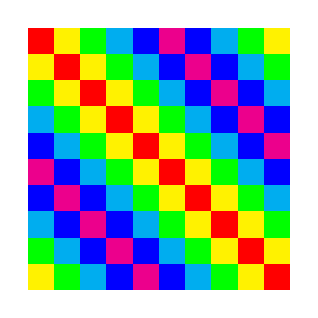
\begin{tikzpicture}[scale = 0.333333333333333]
        \fill[red] (0, 9) rectangle (1, 10);
        \fill[yellow] (1, 9) rectangle (2, 10);
        \fill[green] (2, 9) rectangle (3, 10);
        \fill[cyan] (3, 9) rectangle (4, 10);
        \fill[blue] (4, 9) rectangle (5, 10);
        \fill[magenta] (5, 9) rectangle (6, 10);
        \fill[blue] (6, 9) rectangle (7, 10);
        \fill[cyan] (7, 9) rectangle (8, 10);
        \fill[green] (8, 9) rectangle (9, 10);
        \fill[yellow] (9, 9) rectangle (10, 10);
        \fill[yellow] (0, 8) rectangle (1, 9);
        \fill[red] (1, 8) rectangle (2, 9);
        \fill[yellow] (2, 8) rectangle (3, 9);
        \fill[green] (3, 8) rectangle (4, 9);
        \fill[cyan] (4, 8) rectangle (5, 9);
        \fill[blue] (5, 8) rectangle (6, 9);
        \fill[magenta] (6, 8) rectangle (7, 9);
        \fill[blue] (7, 8) rectangle (8, 9);
        \fill[cyan] (8, 8) rectangle (9, 9);
        \fill[green] (9, 8) rectangle (10, 9);
        \fill[green] (0, 7) rectangle (1, 8);
        \fill[yellow] (1, 7) rectangle (2, 8);
        \fill[red] (2, 7) rectangle (3, 8);
        \fill[yellow] (3, 7) rectangle (4, 8);
        \fill[green] (4, 7) rectangle (5, 8);
        \fill[cyan] (5, 7) rectangle (6, 8);
        \fill[blue] (6, 7) rectangle (7, 8);
        \fill[magenta] (7, 7) rectangle (8, 8);
        \fill[blue] (8, 7) rectangle (9, 8);
        \fill[cyan] (9, 7) rectangle (10, 8);
        \fill[cyan] (0, 6) rectangle (1, 7);
        \fill[green] (1, 6) rectangle (2, 7);
        \fill[yellow] (2, 6) rectangle (3, 7);
        \fill[red] (3, 6) rectangle (4, 7);
        \fill[yellow] (4, 6) rectangle (5, 7);
        \fill[green] (5, 6) rectangle (6, 7);
        \fill[cyan] (6, 6) rectangle (7, 7);
        \fill[blue] (7, 6) rectangle (8, 7);
        \fill[magenta] (8, 6) rectangle (9, 7);
        \fill[blue] (9, 6) rectangle (10, 7);
        \fill[blue] (0, 5) rectangle (1, 6);
        \fill[cyan] (1, 5) rectangle (2, 6);
        \fill[green] (2, 5) rectangle (3, 6);
        \fill[yellow] (3, 5) rectangle (4, 6);
        \fill[red] (4, 5) rectangle (5, 6);
        \fill[yellow] (5, 5) rectangle (6, 6);
        \fill[green] (6, 5) rectangle (7, 6);
        \fill[cyan] (7, 5) rectangle (8, 6);
        \fill[blue] (8, 5) rectangle (9, 6);
        \fill[magenta] (9, 5) rectangle (10, 6);
        \fill[magenta] (0, 4) rectangle (1, 5);
        \fill[blue] (1, 4) rectangle (2, 5);
        \fill[cyan] (2, 4) rectangle (3, 5);
        \fill[green] (3, 4) rectangle (4, 5);
        \fill[yellow] (4, 4) rectangle (5, 5);
        \fill[red] (5, 4) rectangle (6, 5);
        \fill[yellow] (6, 4) rectangle (7, 5);
        \fill[green] (7, 4) rectangle (8, 5);
        \fill[cyan] (8, 4) rectangle (9, 5);
        \fill[blue] (9, 4) rectangle (10, 5);
        \fill[blue] (0, 3) rectangle (1, 4);
        \fill[magenta] (1, 3) rectangle (2, 4);
        \fill[blue] (2, 3) rectangle (3, 4);
        \fill[cyan] (3, 3) rectangle (4, 4);
        \fill[green] (4, 3) rectangle (5, 4);
        \fill[yellow] (5, 3) rectangle (6, 4);
        \fill[red] (6, 3) rectangle (7, 4);
        \fill[yellow] (7, 3) rectangle (8, 4);
        \fill[green] (8, 3) rectangle (9, 4);
        \fill[cyan] (9, 3) rectangle (10, 4);
        \fill[cyan] (0, 2) rectangle (1, 3);
        \fill[blue] (1, 2) rectangle (2, 3);
        \fill[magenta] (2, 2) rectangle (3, 3);
        \fill[blue] (3, 2) rectangle (4, 3);
        \fill[cyan] (4, 2) rectangle (5, 3);
        \fill[green] (5, 2) rectangle (6, 3);
        \fill[yellow] (6, 2) rectangle (7, 3);
        \fill[red] (7, 2) rectangle (8, 3);
        \fill[yellow] (8, 2) rectangle (9, 3);
        \fill[green] (9, 2) rectangle (10, 3);
        \fill[green] (0, 1) rectangle (1, 2);
        \fill[cyan] (1, 1) rectangle (2, 2);
        \fill[blue] (2, 1) rectangle (3, 2);
        \fill[magenta] (3, 1) rectangle (4, 2);
        \fill[blue] (4, 1) rectangle (5, 2);
        \fill[cyan] (5, 1) rectangle (6, 2);
        \fill[green] (6, 1) rectangle (7, 2);
        \fill[yellow] (7, 1) rectangle (8, 2);
        \fill[red] (8, 1) rectangle (9, 2);
        \fill[yellow] (9, 1) rectangle (10, 2);
        \fill[yellow] (0, 0) rectangle (1, 1);
        \fill[green] (1, 0) rectangle (2, 1);
        \fill[cyan] (2, 0) rectangle (3, 1);
        \fill[blue] (3, 0) rectangle (4, 1);
        \fill[magenta] (4, 0) rectangle (5, 1);
        \fill[blue] (5, 0) rectangle (6, 1);
        \fill[cyan] (6, 0) rectangle (7, 1);
        \fill[green] (7, 0) rectangle (8, 1);
        \fill[yellow] (8, 0) rectangle (9, 1);
        \fill[red] (9, 0) rectangle (10, 1);
    \end{tikzpicture}
    \caption[Vizualizacija matrica \ensuremath{P} i \ensuremath{Q}]{Vizualizacija matrica \ensuremath{P} i \ensuremath{Q}. U ovom je slučaju \ensuremath{k = \numprint{10}} i vrijednosti \ensuremath{p_{i}} odnosno \ensuremath{q_{i}} za \ensuremath{i \in \left\{ \numprint{0} , \numprint{1} , \dotsc , \numprint{5} \right\}} obojane su s obzirom na indeks \ensuremath{i}, a ne s obzirom na vrijednost za neki konkretni početni niz \ensuremath{a_{\numprint{1}} , a_{\numprint{2}} , \dotsc , a_{\numprint{10}}}.}
    \label{fig:matrix_P_visualisation}
\end{figure}

\par

\subsection{Karakterizacija trokuta}

Neka je $ T \subseteq \reals^{\numprint{2}} $ proizvoljni trokut. Njegova svaka dva (različita) vrha razapinju jednu njegovu stranicu, stoga po propoziciji~\ref{prop:diameter_polygon} postoji jedna njegova stranica koja je dugačaka onoliko koliko iznosi dijametar trokuta $ T $. Sada taj trokut možemo skalirati s $ d^{{- \numprint{1}}} \left( T \right) $, rotirati i translatirati tako da novi (ali početnom trokutu $ T $ sličan) trokut $ T ' $ \emph{leži} na dužini $ \linesegment{\left( {- \frac{\numprint{1}}{\numprint{2}}} , \numprint{0} \right)}{\left( \frac{\numprint{1}}{\numprint{2}} , \numprint{0} \right)} $ i da mu je treći vrh sa strogo pozitivnom drugom koordinatom. Ako, pak, taj treći vrh trokuta $ T ' $ ima strogo negativnu prvu koordinatu, onda konstruiramo trokut $ T '' $ dobiven refleksijom trokuta $ T ' $ oko ordinate (inače možemo uzeti $ T '' = T ' $). Time smo dobili trokut sličan početnom trokutu čije su dvije točke fiksne, a za treću znamo da se nalazi u prvom kvadrantu (uključujući koordinatne osi, to jest, uključujući ordinatu) i taj dobiveni trokut je dijametra $ \numprint{1} $.

\par

Označimo onaj treći, \emph{varijabilni} vrh trokuta $ T '' $ s $ \left( x_{T ''} , y_{T ''} \right) \in \reals^{\numprint{2}} $. Tada je
\begin{equation*}
    \distance{\left( \frac{\numprint{1}}{\numprint{2}} , \numprint{0} \right)}{\left( x_{T ''} , y_{T ''} \right)} \leq \distance{\left( {- \frac{\numprint{1}}{\numprint{2}}} , \numprint{0} \right)}{\left( x_{T ''} , y_{T ''} \right)} \leq \numprint{1}
\end{equation*}
(prva nejednakost posljedica je činjenice da je $ x_{T ''} \geq \numprint{0} $, a druga činjenice da je $ \diameter \left( T '' \right) = \numprint{1} $. Kvadriranjem i raspisivanjem izraza za euklidsku udaljenost dobijemo
\begin{equation*}
    \left( x_{T ''} + \frac{\numprint{1}}{\numprint{2}} \right)^{\numprint{2}} + y_{T ''}^{\numprint{2}} \leq \numprint{1} \text{,}
\end{equation*}
to jest, $ \left( x_{T ''} , y_{T ''} \right) $ je u presjeku prvog kvadranta (uključujući strogo pozitivni dio ordinate) i zatvorenog kruga radijusa $ \numprint{1} $ sa središtem u točki $ \left( {- \frac{\numprint{1}}{\numprint{2}}} , \numprint{0} \right) $. Ovo možemo dalje raspisati kao
\begin{align*}
    \numprint{0} & \leq x_{T ''} < \frac{\numprint{1}}{\numprint{2}} \text{,} & \numprint{0} < y_{T ''} & \leq \sqrt{\frac{\numprint{3}}{\numprint{4}} - x_{T ''} - x_{T ''}^{\numprint{2}}}
\end{align*}
(donje ograde posljedica su činjenice da je taj vrh u prvom kvadrantu uključujući strogo pozitivni dio ordinate). Kada bi bilo $ x_{T ''} = \frac{\numprint{1}}{\numprint{2}} $, onda bi zbog donje ograde vrijedilo $ y_{T ''} > \numprint{0} $, a zbog gornje ograde $ y_{T ''} \leq \numprint{0} $---to je kontradijkcija, dakle, vrijedi $ x_{T ''} \neq \frac{\numprint{1}}{\numprint{2}} $.

\par

Uočimo, također, da je taj treći vrh jedinstveno određen. Naime, na jednakokračnim trokutima kojima je baza veća od krakova (uključujući jednakostranični trokut) postojale bi dvije opcije, ali one bi, zapravo, bile jednake---treći vrh \emph{ležao} bi na ordinati. U svim drugim slučajevima druge su dvije stranice (koje nisu dužina $ \linesegment{\left( {- \frac{\numprint{1}}{\numprint{2}}} , \numprint{0} \right)}{\left( \frac{\numprint{1}}{\numprint{2}} , \numprint{0} \right)} $) različitih duljina, stoga samo u jednom položaju taj treći vrh može biti u prvom kvadrantu. Jednakokračni trokuti kojima je krak dulji od baze, kao i svi jednakokračni trokuti, simetrični su s obzirom na simetralu baze, stoga je svejedno koji krak \emph{polegnemo} na dužinu $ \linesegment{\left( {- \frac{\numprint{1}}{\numprint{2}}} , \numprint{0} \right)}{\left( \frac{\numprint{1}}{\numprint{2}} , \numprint{0} \right)} $.

\par

Lako se provjeri i da proizvoljna točka $ \left( x , y \right) \in \reals^{\numprint{2}} $ za koju je $ \numprint{0} \leq x < \frac{\numprint{1}}{\numprint{2}} $ i $ \numprint{0} < y \leq \sqrt{\frac{\numprint{3}}{\numprint{4}} - x - x^{\numprint{2}}} $ s točkama $ \left( {\pm \frac{\numprint{1}}{\numprint{2}}} , \numprint{0} \right) $ zadaje trokut dijametra $ \numprint{1} $. Iz svega navedenog slijedi propozicija~\ref{prop:triangle_characteristic_bijective} (injektivnost je posljedica definicije relacije ekvivalencije sličnosti---\seetxt~definiciju~\ref{def:similarity}).

\par

\begin{proposition} \label{prop:triangle_characteristic_bijective}
    Označimo skup svih klasa sličnosti otvorenih trokuta u ravnini sa $ S_{{\bigtriangleup}} \subseteq \powerset \left( \reals^{\numprint{2}} \right) $ i
    \begin{equation*}
        D_{{\bigtriangleup}} \coloneqq \left\{ \left( x , y \right) \in \reals^{\numprint{2}} : \numprint{0} \leq x < \frac{\numprint{1}}{\numprint{2}} \land \numprint{0} < y \leq \sqrt{\frac{\numprint{3}}{\numprint{4}} - x - x^{\numprint{2}}} \right\} \subseteq \reals^{\numprint{2}} \text{.}
    \end{equation*}
    Tada je preslikavanje $ C \colon S_{{\bigtriangleup}} \to D_{{\bigtriangleup}} $ definirano tako da klasi $ T \in S_{{\bigtriangleup}} $ pridružuje onu točku $ V \in D_{{\bigtriangleup}} $ za koju postoji trokut u klasi $ T $ čiji su vrhovi $ \left( \frac{\numprint{1}}{\numprint{2}} , \numprint{0} \right) , V , \left( {- \frac{\numprint{1}}{\numprint{2}}} , \numprint{0} \right) $ dobro definirano i ono je bijektivno.
\end{proposition}

\par

\begin{figure}[htb!]
    \centering
    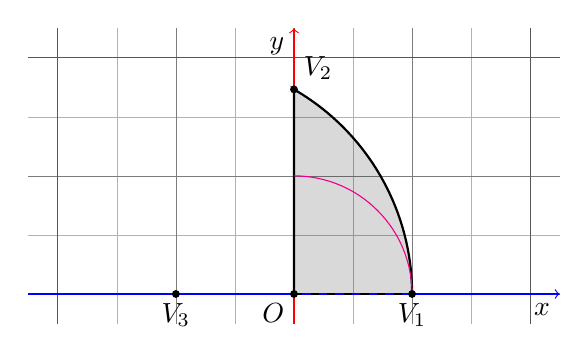
\begin{tikzpicture}[scale = 3]
        % Koordinatna mreza.
        \draw[black, opacity = 0.3, very thin, step = 0.25] (-1.125, -0.125) grid (1.125, 1.125);
        \draw[black, opacity = 0.3, very thin, step = 0.5] (-1.125, -0.125) grid (1.125, 1.125);
        \draw[black, opacity = 0.3, thin, step = 1] (-1.125, -0.125) grid (1.125, 1.125);

        % Koordinatne osi.
        \draw[blue, thin, ->] (-1.125, 0) -- (1.125, 0) node[black, below left] {$ x $};
        \draw[red, thin, ->] (0, -0.125) -- (0, 1.125) node[black, below left] {$ y $};

        % Skup S_\bigtriangleup^1.
        \fill[black, opacity = 0.15] (0.5, 0) arc (0:60:1) -- (0, 0.866025403784439) -- (0, 0) -- cycle;

        % Rub skupa S_\bigtriangleup^*.
        \draw[black, thick, dashed] (0, 0) -- (0.5, 0);
        \draw[black, thick] (0.5, 0) arc (0:60:1) -- (0, 0.866025403784439) -- (0, 0);

        % Slika pravokutnih trokuta.
        \draw[magenta] (0.5, 0) arc (0:90:0.5);

        % Ishodiste.
        \fill[black] (0, 0) circle (0.016666666666667) node[below left] {$ O $};

        % Vrhovi jednakostranicnog trokuta.
        \fill[black] (0.5, 0) circle (0.016666666666667) node[below] {$ V_{\numprint{1}} $};
        \fill[black] (0, 0.866025403784439) circle (0.016666666666667) node[above right] {$ V_{\numprint{2}} $};
        \fill[black] (-0.5, 0) circle (0.016666666666667) node[below] {$ V_{\numprint{3}} $};
    \end{tikzpicture}
    \caption[Skup \ensuremath{D_{{\bigtriangleup}}} iz propozicije~\ref{prop:triangle_characteristic_bijective}]{Skup \ensuremath{D_{\bigtriangleup}} iz propozicije~\ref{prop:triangle_characteristic_bijective}. Koordinate točaka su: ishodište \ensuremath{O = \left( \numprint{0} , \numprint{0} \right)}, vrhovi jednakostraničnog trokuta \ensuremath{V_{\numprint{1}} = \left( \frac{\numprint{1}}{\numprint{2}} , \numprint{0} \right) , V_{\numprint{2}} = \left( \numprint{0} , \frac{\sqrt{\numprint{3}}}{\numprint{2}} \right) , V_{\numprint{3}} = \left( {- \frac{\numprint{1}}{\numprint{2}}} , \numprint{0} \right)}. Purpurnocrveni luk sjecište je skupa \ensuremath{D_{{\bigtriangleup}}} i kružnice radijusa \ensuremath{\frac{\numprint{1}}{\numprint{2}}} sa središtem u ishodištu, a predstavlja one točke u koje se preslikavaju pravokutni trokuti.}
    \label{fig:triangle_characteristic_region}
\end{figure}

\par

Skup $ D_{{\bigtriangleup}} $ iz propozicije~\ref{prop:triangle_characteristic_bijective} ilustriran je na slici~\ref{fig:triangle_characteristic_region}. Na rubu tog skupa (bez apscise) točke su u koje se preslikavaju jednakokračni trokuti: na kružni luk oni jednakokračni trokuti kojima je baza kraća od krakova, a na ordinatu oni kojima je baza dulja od krakova. Na sjecište tih dijelova ruba---u točku $ \left( \numprint{0} , \frac{\sqrt{\numprint{3}}}{\numprint{2}} \right) $---preslikavaju se jednakostranični trokuti koji su, zapravo, jednakokračni trokuti kojima je baza jednake duljine kao i krakovi. Na slici~\ref{fig:triangle_characteristic_region} dodatno je označen i luk na koji se preslikavaju svi pravokutni trokuti. \emph{Iznad} tog luka preslikavaju se šiljastokutni trokuti, a \emph{ispod} tupokutni.

\par

Za dani trokut zapravo nije potrebno tražiti sličnost kojom se njegova karakterizacija iz propozicije~\ref{prop:triangle_characteristic_bijective} može \emph{iščitati} iz koordinata trećeg vrha. Naime, ako je udaljenost polovišta najdulje stranice i ortogonalne projekcije vrha nasuprot najdulje stranice na nju jednaka $ x \in \intervaloo{0}{{+ \infty}} $, a visina trokuta iznad najdulje stranice jednaka $ y \in \intervaloo{0}{{+ \infty}} $, onda se taj trokut preslikava u $ d^{{- 1}} \left( x , y \right) $, gdje je $ d \in \intervaloo{0}{{+ \infty}} $ dijametar trokuta, to jest, duljina njegove najdulje stranice. Štoviše, ako su duljine stranice trokuta $ a , b , c \in \intervaloo{0}{{+ \infty}} $ tako da je $ a \geq c \geq b $, i ako su unutarnji kutovi trokuta $ \alpha , \beta , \gamma \in \intervaloo{0}{\pi} $ redom nasuprot stranica $ a , b , c $, onda se taj trokut preslikava u točku $ \left( \frac{1}{2} - \frac{b}{a} \cos \gamma  , \frac{b}{a} \sin \gamma \right) $. Opisano se, naime, može vidjeti na slici~\ref{fig:triangle_characteristic_region}.

\par

Karakterizacija trokuta kao u propoziciji~\ref{prop:triangle_characteristic_bijective} zapravo je karakterizacija poligona iz teorema~\ref{thm:polygon_unique_vertices} uz prethodne transformacije. Slične je karakterizacije moguće definirati i za ostale poligone: na primjer, u točke $ \left( {\pm \frac{\numprint{1}}{\numprint{2}}} , \numprint{0} \right) $ preslikamo (preko neke sličnosti) vrhove početnog poligona čija je udaljenost jednaka dijametru tog poligona (\seetxt~propoziciju~\ref{prop:diameter_polygon}), i to tako da je uređena $ k $-torka koordinata vrhova rezultantnog poligona u pozitivnom smjeru počevši od vrha $ \left( \frac{\numprint{1}}{\numprint{2}} , \numprint{0} \right) $ leksikografski najveća.

\par

\subsection{Vizualna karakterizacija poligona}

Možda je najjednostavnija karakterizacija poligona \emph{vizualna}---u \emph{nematematičkom} svijetu nekome određeni poligon možemo objasniti tako da mu pokažemo kako on izgleda (nacrtamo ga ili mu damo, na primjer, papir izrezan u obliku tog poligona). Slično kao što su ilustracije \emph{riješene} na zaslonima s pikselima, ovu karakterizaciju možemo definirati i matematički.

\par

Neka je poligon $ P \subseteq \reals^{\numprint{2}} $ proizvoljan. Neka su $ x_{{\min}} , x_{{\max}} , y_{{\min}} , y_{{\max}} \in \reals $ proizvoljni takvi da za svaku točku $ \left( x , y \right) \in \closure{P} $ vrijedi $ x_{{\min}} \leq x \leq x_{{\max}} $ i $ y_{{\min}} \leq y \leq y_{{\min}} $. Neka su $ m , n \in \positives{\naturals} $ proizvoljni. Označimo
\begin{equation*}
    h_{x} \coloneqq \frac{x_{{\max}} - x_{{\min}}}{m} , h_{y} \coloneqq \frac{y_{{\max}} - y_{{\min}}}{n} \in \intervaloo{\numprint{0}}{{+ \infty}} \text{.}
\end{equation*}
Nadalje, za $ i \in \left\{ \numprint{0} , \numprint{1} , \dotsc , m \right\} $ označimo $ x_{i} \coloneqq x_{{\min}} + i h_{x} $, a za $ j \in \left\{ \numprint{0} , \numprint{1} , \dotsc , n \right\} $ označimo $ y_{j} \coloneqq y_{{\min}} + j h_{y} $. Ovime je zapravo napravljena ekvidistantna mreža pravokutnika $ \intervalcc{x_{{\min}}}{x_{{\max}}} \times \intervalcc{y_{{\min}}}{y_{{\max}}} $ koja na prvoj koordinati ima $ m $ dijelova, a na drugoj $ n $. U tom pravokutniku leži cijeli poligon $ P $.

\par

Za svake $ \left( i , j \right) \in \left\{ \numprint{1} , \numprint{2} , \dotsc , m \right\} \times \left\{ \numprint{1} , \numprint{2} , \dotsc , n \right\} $ definiramo vrijednost $ a_{i j} \geq \numprint{0} $ kao površinu presjeka $ \left( \intervalcc{x_{i - \numprint{1}}}{x_{i}} \times \intervalcc{y_{j - \numprint{1}}}{y_{j}} \right) \cap P $ podijeljenu s $ h_{x} h_{y} $ ($ \numprint{0} $ ako je taj presjek prazan). Ove definirane normirane površine možemo spojiti u matricu $ \asmatrix{A} \coloneqq \left( a_{i j} \right) \in \MatrixAlgebramn{\reals}{m}{n} $ čiji su svi elementi tada u intervalu $ \intervalcc{\numprint{0}}{\numprint{1}} $.

\par

Budući da je rub poligona po definiciji \emph{sastavljen} od konačno mnogo dužina, svaki od elemenata matrice $ h_{x} h_{y} \asmatrix{A} $ možemo izračunati kao aritmetički izraz koordinata vrhova poligona $ P $ i vrijednosti ekvidistantne diskretizacije. Neprekidnost tih aritmetičkih izraza s obzirom na varijable implicira neprekidnost matrice $ h_{x} h_{y} \asmatrix{A} $ s obzirom na koordinate vrhova (dokle god je cijeli poligon sadržan u ekvidistantnoj mreži), dakle, neprekidna je i matrica $ \asmatrix{A} $. Međutim, ona nije robusna na rotacije i refleksije (invarijantnost na translacije i skaliranje možemo postići korigiranjem rubova i koraka $ h_{x} , h_{y} $ ekvidistantne mreže).

\par

Kada bismo pravokutnike u ekvidistantnoj mreži bojali ovisno o vrijednosti odgovarajućeg elementa matrice $ \asmatrix{A} $ tako da je, na primjer, $ \numprint{0} $ obojano crnom, $ \numprint{1} $ bijelom, a da između nijansa sive linearno raste od crne u $ \numprint{0} $ do bijele u $ \numprint{1} $, onda bi ta slika \emph{ličila} početnom poligonu. Primjer se može vidjeti na slici~\ref{fig:triangle_mesh}. Što je ekvidistantna mreža finija (što su $ h_{x} , h_{y} $ manji, to jest, što su $ m , n $ veći), to će slika biti reprezentativnija. Na računalima se, u $ \numprint{8} $-bitnim bojama, poligoni na ovaj način na zaslonu prikazuju tako da se na pikselu koji reprezentira jedno polje mreže nijansa sive računa kao najbliži cijeli broj broju $ \numprint{255} a_{i j} $ s odgovarajućim indeksima $ i , j $.

\par

\begin{figure}[htb!]
    \centering
    \begin{subfigure}{0.45\textwidth}
        \centering
        {%
            \setlength{\fboxsep}{0pt}%
            \setlength{\fboxrule}{1pt}%
            \fcolorbox{red}{white}{
\includegraphics{figures/triangle_mesh.png}}%
        }
        \caption{Cijeli trokut}
        \label{fig:triangle_mesh_complete}
    \end{subfigure}
    \begin{subfigure}{0.45\textwidth}
        \centering
        {%
            \setlength{\fboxsep}{0pt}%
            \setlength{\fboxrule}{1pt}%
            \fcolorbox{red}{white}{
\includegraphics{figures/triangle_mesh_zoom.png}}%
        }
        \caption{Dio uz rub trokuta}
        \label{fig:triangle_mesh_zoom}
    \end{subfigure}
    \caption{Vizualizacija trokuta}
    \label{fig:triangle_mesh}
\end{figure}

\par

Primijetimo da u opisanoj karakterizaciji, ako za neki element $ a_{i j} $ znamo da je jednak $ \numprint{1} $, onda ne znamo koliko je odgovarajući pravokutnik (čija je normirana površina presjeka s $ P $ izražena elementom $ a_{i j} $) udaljen od ruba poligona $ P $. Takva bi informacija, doduše, kod rješavanja diferencijalne zadaće~\eqref{eq:Dirichlet_Laplacian_problem} bila korisna zbog rubnog uvjeta. Donekle \emph{informativnija} karakterizacija može se dobiti pomoću funkcije dubine iz definicije~\ref{def:set_deepness}.

\par

\begin{definition} \label{def:set_deepness}
    Neka je $ n \in \positives{\naturals} $. Neka je $ S \subseteq \reals^{n} $. Funkciju $ \deepness_{S} \colon \reals^{n} \to \intervalcc{\numprint{0}}{{+ \infty}} $ definiranu s
    \begin{equation}
        \deepness_{S} \left( x \right) =
        \begin{cases}
            \distance{x}{\boundary S} & x \in \interior S \text{,} \\
            \numprint{0} & \text{inače}
        \end{cases}
        , \quad \forall x \in \reals^{n} \text{,}
    \end{equation}
    gdje je $ \distance{x}{\boundary S} = \inf \left( \left\{ \distance{x}{y} \in \intervalco{\numprint{0}}{{+ \infty}} : y \in \boundary S \right\} \right) $ po refleksivnom uređaju ($ \distance{x}{\boundary S} = {+ \infty} $ ako je $ \boundary S = \emptyset $), za svaki $ x \in \reals^{n} $, zovemo \defined{funkcijom dubine} odnosno \defined{dubinom skupa $ S $}.
\end{definition}

\par

Kao što je gore definirana matrica $ \asmatrix{A} $, isto tako možemo definirati matricu $ \asmatrix{B} \in \MatrixAlgebramn{\reals}{m}{n} $ čiji elementi su definirani s $ b_{i j} = \deepness_{P} \left( x_{i - \numprint{1}} + \frac{h_{x}}{\numprint{2}} , y_{j - \numprint{1}} + \frac{h_{y}}{\numprint{2}} \right) $ (točka $ \left( x_{i - \numprint{1}} + \frac{h_{x}}{\numprint{2}} , y_{j - \numprint{1}} + \frac{h_{y}}{\numprint{2}} \right) \in \reals^{2} $ na sjecištu je dijagonala pravokutnika $ \intervalcc{x_{i - \numprint{1}}}{x_{i}} \times \intervalcc{y_{j - \numprint{1}}}{y_{j}} $, dakle, na njegovoj je sredini). Da bismo tako dobivenu matricu \emph{obojali} kao što je gore opisano bojanje matrice $ \asmatrix{A} $, ove vrijednosti potrebno je prvo normirati---na primjer, tako da ih podijelimo s dijametrom poligona $ P $ ili s maksimumom funkcije dubine---jer funkcija dubine može poprimati proizvoljno velike vrijednosti (ovisno o poligonu i njegovu dijametru). Primjer \emph{bojanja} takve matrice na nekom trokutu normiranjem po maksimumu prikazan je na slici~\ref{fig:triangle_deepness}.

\par

\begin{figure}[htb!]
    \centering
    {%
        \setlength{\fboxsep}{0pt}%
        \setlength{\fboxrule}{1pt}%
        \fcolorbox{red}{white}{
\includegraphics{figures/triangle_deepness.png}}%
    }
    \caption[Vizualizacija funkcije dubine trokuta]{Vizualizacija funkcije dubine trokuta. Dubina je normirana tako da maksimum koji poprima iznosi \ensuremath{\numprint{1}}.}
    \label{fig:triangle_deepness}
\end{figure}

\par

I karakterizacija poligona matricom $ \asmatrix{B} $ pomoću funkcije dubine je neprekidna. Njezina neprekidnost proizlazi iz činjenice da je udaljenost točaka neprekidna, da je udaljenost svake točke na rubu skupa od ruba skupa jednaka $ \numprint{0} $ (točka na rubu je za $ \numprint{0} $ udaljena od same sebe, što je, dakle, infimum udaljenosti od točaka na rubu), a, da bi se iz eksteriora skupa \emph{prešlo} u interior i obratno, potrebno je prijeći rub skupa.

\par

Obje opisane karakterizacije mogu rezultirati istim matricama za različite poligone ako diskretizacija nije dovoljno \emph{fina}. No, za dovoljno \emph{finu} diskretizaciju, čak i ako dva različita poligona imaju istu karakterizaciju, u pronalasku numeričkog rješenja diferencijalne jednadžbe~\eqref{eq:Dirichlet_Laplacian_problem} to ne predstavlja problem zbog neprekidnosti rješenja s obzirom na oblik domene (\seetxt~teorem~\ref{thm:Laplace_eigenvalue_continuity}). To jest, ako su dva poligona neznatno različiti (u nekom kontekstu), onda su i svojstvene vrijednosti Laplaceovog operatora na tim poligonima koje nas zanimaju također zanemarivo različite pa u njihovu računanju razliku između poligona možemo zanemariti.

\par
